\documentclass[11pt]{report}

\usepackage[utf8]{inputenc}
\usepackage[T1]{fontenc}
\usepackage[french]{babel}
\usepackage{mathptmx}
\usepackage{graphicx}  % sans draft = les vraies images sont affichées
\usepackage{geometry}
\geometry{top=2.5cm,bottom=2.5cm,left=2.5cm,right=2.5cm}
\usepackage{setspace}
\singlespacing
\usepackage{color}
\usepackage{indentfirst}
\setlength{\parindent}{1.25cm}
\setlength{\parskip}{0.35em}
\usepackage{titling}
\usepackage{tikz}
\usepackage{float}
\usepackage{array}
\usepackage{tabularx}
\usepackage{multirow}
\usepackage{url}
\usepackage{enumitem}
\usepackage{csquotes}
\usepackage[most]{tcolorbox}
\usepackage{hyperref}
\usepackage[nohints]{minitoc}
\AtBeginEnvironment{thebibliography}{\raggedright}

\newcommand{\roundedimage}[2][\textwidth]{%
    \begin{tcolorbox}[
        enhanced,
        width=\dimexpr#1+10pt\relax,
        colframe=gray!75,
        colback=white,
        boxrule=1pt,
        arc=2pt,
        outer arc=2pt,
        boxsep=4pt,
        left=0pt,
        right=0pt,
        top=0pt,
        bottom=0pt,
        before skip=0pt,
        after skip=0pt
    ]
        \centering
        \includegraphics[width=#1]{#2}
    \end{tcolorbox}%
}

\newcommand{\roundedfullwidthimage}[1]{%
    \begin{tcolorbox}[
        enhanced,
        width=\textwidth,
        colframe=gray!75,
        colback=white,
        boxrule=1pt,
        arc=2pt,
        outer arc=2pt,
        boxsep=4pt,
        left=0pt,
        right=0pt,
        top=0pt,
        bottom=0pt,
        before skip=0pt,
        after skip=0pt
    ]
        \centering
        \includegraphics[width=\dimexpr\textwidth-10pt\relax]{#1}
    \end{tcolorbox}%
}




%==========================================%
%==========================================%
\newcommand*{\blankpage}{%
	\vspace*{\fill}
	{\centering This page intentionally left blank. \par}
	\vspace{\fill}}
\makeatletter
\renewcommand*{\cleardoublepage}{\clearpage\if@twoside \ifodd\c@page\else
	\blankpage
	\thispagestyle{empty}
	\newpage
	\if@twocolumn\hbox{}\newpage\fi\fi\fi}
\makeatother
%__________________________________________%
%__________________________________________%
\renewcommand{\mtctitle}{Sommaire}
% \setcounter{minitocdepth}{2}
\dominitoc
\newcommand{\titresection}[1]{%
  \vspace{1.5em}%
  {\LARGE\bfseries #1}\par%
  \vspace{0.5em}%
}

\begin{document}

\thispagestyle{empty}

% === Logos en haut ===
\noindent
\begin{minipage}[t]{0.45\textwidth}
    
\includegraphics[draft=false,width=4.2cm]{logos/logo-ISIS-horizontal-RVB-HD.png}
\end{minipage}
\hfill
\begin{minipage}[t]{0.45\textwidth}
    \raggedleft
    
\includegraphics[draft=false,width=5.5cm]{logos/Logo_Pierre_Fabre_67a4d7cd39e89ab3a67a7c3e41ea3d7d.png.jpg}
\end{minipage}

\vspace{2.5cm}

% === Bloc central : titre + infos ===
\begin{center}
    {\Huge \textbf{Rapport d'ingénierie}}\\[0.8cm]
    \rule{\linewidth}{0.4pt}
    \vspace{0.4cm}

    {\LARGE \textbf{Raw Material Insight : étude d'un système d'aide à la décision pour la R\&D}}\\

    \vspace{0.4cm}
    \rule{\linewidth}{0.4pt}
    \vspace{0.8cm}

    {\Large \textit{Laboratoires Pierre Fabre — R\&D DCPC}}\\[0.4cm]
    \normalsize
    \vspace{0.6cm}
    \textbf{Année universitaire :} 2025--2026\\
    \vspace{0.3cm}
    \textbf{Période :} du 20 décembre 2025 au 1er septembre 2026
\end{center}

\vspace{2cm}

% === Bas de page ===
\begin{flushleft}
    \textbf{Apprentie :} Inès GRIBAA \hfill \textit{FIA 4 Promotion 2027} \\[0.2cm]
    \textbf{Maître d'apprentissage :} Laurent LASBENNES \\[0.2cm]
    \textbf{Tuteur pédagogique :} Elyes LAMINE
\end{flushleft}

\clearpage
 % Uncomment this line to include the cover page
%\clearpage
\pagenumbering{roman}	

%\blankpage
%__________________frontmatter______________%
\clearpage
\thispagestyle{empty}

% En-tête avec logo et titre alignés
\vspace*{0.8cm}
\begin{minipage}{0.35\textwidth}
    
\includegraphics[draft=false,width=4cm]{logos/logo-ISIS-horizontal-RVB-HD.png}
\end{minipage}
\hfill
\begin{minipage}{0.6\textwidth}
    \centering
    {\bfseries\large Rapport d'alternance : Visa du maître d'apprentissage}
\end{minipage}

\vspace{1cm}
\hrule
\vspace{1.5cm}

% Interligne augmenté globalement
\renewcommand{\baselinestretch}{1.4}\selectfont

% Informations entreprise
\noindent
\textbf{Établissement :} Laboratoires Pierre Fabre\\
\textbf{Nom et prénom :} Laurent LASBENNES \\

\vspace{1.8cm}

% Bloc central
\begin{center}
    \textbf{\textit{a pris connaissance du rapport d'alternance de l'apprentie :}}
\end{center}

\vspace{1.8cm}

\noindent
\textbf{Nom et prénom :} Inès GRIBAA \\
\textbf{Promotion :} 2027 \\
\textbf{Titre du rapport :} Appui à la structuration d'un outil de gestion de cohorte \\
\textbf{Année universitaire :} 2025--2026

\vspace{2.5cm}

\vspace{1cm}

\noindent
\hspace*{4cm}
Fait à \makebox[2cm]{\dotfill} \hspace{1cm} Le \makebox[5cm]{\dotfill}

\vspace*{1cm}
\noindent
\hfill \textbf{Signature}

\clearpage

 
%\input{./frontmatter/page_signaletique}
\begin{titlepage}
\titresection{Résumé}

\vspace{0.75cm}
\begin{spacing}{1}
Le présent rapport analyse Raw Material Insight, un système d’aide à la décision développé au sein de la R\& D Pierre Fabre pour la gestion stratégique des matières premières. Face à la complexité croissante des exigences réglementaires, à l’augmentation continue du nombre de matières premières utilisées dans les formules et au besoin de sécuriser les processus industriels, l’entreprise a mis en place un système multi-source permettant de consolider les données du PLM, des spinners, des statistiques de ventes (SDV), de la Data Marketplace et d’outils internes tels que SharePoint.
Raw Material Insight fournit une vision synthétique et hiérarchisée du portefeuille matières, identifie les dossiers nécessitant une revue, calcule l’impact économique de chaque matière selon son utilisation en production, et met à disposition des outils de recherche avancés et des fiches techniques consolidées. Construit autour d’un flux ETL Alteryx automatisé et d’une couche décisionnelle BI, il est devenu un point d’entrée central pour différents métiers : homologation, sourcing, analytique, sécurisation et formulation.
Mon rôle dans l’étude du système a consisté en une observation approfondie de son fonctionnement et une compréhension de l’architecture afin de contribuer à la future extension analytique du projet, notamment l’intégration de JMP et la mise en place d’une base de données dédiée aux analytiques.
L’étude présentée dans ce rapport s’inscrit dans les attendus du génie logiciel : analyse du besoin, modélisation des données, étude des flux de production et présentation des modalités de mise en production.


\vspace{0.5em}
\end{spacing}

\vspace{2em}

\titresection{Abstract}


\vspace{0.75cm}
\begin{spacing}{1}
This report provides an analysis of Raw Material Insight, a decision-support system developed within Pierre Fabre’s R\&D to enhance the strategic management of raw materials. As regulatory demands increase and the number of raw materials grows, the company needed a multi-source digital system capable of consolidating PLM data, spinners, sales statistics (SDV), the Data Marketplace and internal repositories such as SharePoint.
Raw Material Insight offers a synthetic and prioritized view of the raw material portfolio, identifies dossiers requiring regulatory review, evaluates the economic impact of each material based on production usage, and provides advanced search features and consolidated technical sheets. Built on an automated Alteryx ETL workflow and a BI dashboard layer, the system has become a central tool across several R\& D functions, including homologation, sourcing, analytics, safety and formulation.
My contribution to the project focuses on the observation of the system, the exploration of its data architecture and the preparation for future analytical extensions, particularly through JMP and the construction of an analytical database.
This report follows software engineering methodology: needs analysis, data modeling, production workflow description and implementation details.

\end{spacing}
\end{titlepage}
%\chapter*{Remerciements}
\mtcaddchapter[Remerciements]

\vspace{1em}

Je souhaite remercier toutes les personnes qui m’ont accompagné durant ce stage, réalisé dans le cadre de ma formation à l’École d’ingénieurs ISIS.

Je remercie Madame Sarah Saliou, ma maître de stage, pour le suivi et l'encadrement qu’elle m’a apportés tout au long de ce stage.
Je tiens à remercier aussi Madame Manon Sellos, chargée de projet RI2S, pour ses conseils clairs et son accompagnement tout au long du stage.

Merci également à Rahma Lahriga, pour son aide sur le terrain et les échanges partagés, qui m’ont permis de mieux comprendre les réalités du projet et les besoins exprimés.

Enfin, je remercie Monsieur Sylvain Barreau, mon tuteur pédagogique, pour son suivi, ses conseils et le regard structurant qu’il a apporté à ce travail.

Ce stage m’a offert l’opportunité de mettre en pratique mes compétences dans un contexte réel, en lien direct avec les problématiques de la santé numérique. Il a été une expérience formatrice, tant sur le plan technique que professionnel.


	
%____toc_______________________________________%	
%____toc_______________________________________%	
\tableofcontents
\mtcaddchapter % compense listoffigures pour le compteur minitoc
\newpage
\listoffigures
%\listoftables
\pagenumbering{arabic}
\chapter*{Liste des acronymes}
\addcontentsline{toc}{section}{\textbf{Liste des acronymes} }
  
\begin{spacing}{1.05}

\begin{description}
  \item[MP] \hfill \\
  \textbf{Matière Première} : établissement public de santé regroupant les hôpitaux de Castres et de Mazamet, porteur du programme RI2S.

  \item[MPU] \hfill \\
  \textbf{Matière Première Usine} : programme d’expérimentation visant à tester des solutions numériques pour la santé des seniors en zone rurale.

  \item[MPF] \hfill \\
  \textbf{Matière Première Fournisseur} : interface logicielle permettant à différentes applications ou composants de communiquer entre eux via des appels standards.

  \item[PLM] \hfill \\
  \textbf{Project Life Management} : dispositifs de coordination entre professionnels de santé à l’échelle d’un territoire, pour améliorer la prise en charge des patients.

  \item[ETL] \hfill \\
  \textbf{Extract Transform Load} : langage de feuilles de style utilisé pour décrire la présentation et la mise en forme des pages HTML.

  \item[BI] \hfill \\
  \textbf{Business Intelligence} : langage de balisage standard utilisé pour structurer le contenu d’une page web.

  \item[BU] \hfill \\
  \textbf{Business Unit} : réglementation européenne encadrant le traitement et la circulation des données à caractère personnel.

  \item[DCPC] \hfill \\
  \textbf{DermoCosmétique Personnal Care} : langage de modélisation graphique utilisé pour représenter visuellement la structure, les interactions et le comportement d’un système logiciel.

  \item[UX/UI] \hfill \\
  \textbf{User Experience / User Interface} : ensemble des méthodes visant à optimiser l’ergonomie, l’utilisabilité et l’interface visuelle d’un produit numérique.
\end{description}
\end{spacing}
	
%__________________chapters__________________________________%
\setcounter{minitocdepth}{2}
\chapter*{\textbf{Introduction générale}}
\addstarredchapter{Introduction générale}
\label{intro}
\indent Dans l'industrie pharmaceutique et dermo-cosmétique, la qualité n'est pas un objectif 
parmi d'autres : elle constitue une exigence fondamentale. Les produits développés étant 
destinés à des patients et des consommateurs, leur qualité et leur sécurité doivent être 
maîtrisées tout au long de leur cycle de vie. Cette exigence s'étend aux partenaires et sous
traitants avec lesquels l'entreprise collabore (désignés sous le terme de Tierces Parties dans 
le référentiel qualité du groupe), dont l'évaluation et le suivi participent directement à la maîtrise 
des risques. Cette culture de la qualité est au cœur des activités du groupe Pierre Fabre, 
laboratoire pharmaceutique et dermo-cosmétique français fondé en 1951 à Castres et 
aujourd'hui présent dans 120 pays. 

\indent Assurer le suivi de ces Tierces Parties à grande échelle nécessite de disposer d'une 
donnée fiable, structurée et exploitable. C'est autour de cet enjeu que s'articule IPANEMA. 
Les informations relatives aux Tierces Parties sont collectées à travers une application Power 
Apps et stockées dans différentes listes SharePoint. Jusqu'alors, elles étaient consolidées au 
moyen d'un workflow Alteryx en une table unique, puis restituées dans un dashboard Tableau. 
Cette architecture a cependant révélé plusieurs limites : lignes dupliquées ou manquantes lors 
des jointures, incohérences dans certains calculs et maintenance complexe dans un 
environnement progressivement orienté vers l'écosystème Microsoft.

\indent Le projet a donc consisté à repenser la chaîne de traitement et de valorisation des 
données d'IPANEMA, en construisant un modèle de données adapté et en migrant la partie 
décisionnelle vers Power BI. L'objectif était de proposer aux équipes Qualité une solution plus 
fiable, maintenable et intégrée au système d'information du groupe, leur permettant de 
disposer d'une vision cohérente des informations nécessaires au suivi des Tierces Parties. Au
delà de l'aspect technique, la fiabilisation de ces données contribue ainsi à une meilleure 
maîtrise de la qualité tout au long de la chaîne de valeur.

\indent Ce projet s'inscrit dans ma première année d'alternance au sein de la R&D Dermo
Cosmétique & Personal Care (DCPC) de Pierre Fabre, à Toulouse-Langlade, dans le cadre 
d'un projet démarré en février 2026. En tant que Data Analyst au sein de l'équipe Digital 
Product Dev et Perf, j'ai assuré la conduite du projet IPANEMA dans son ensemble, sous le 
cadrage de mon maître d'apprentissage, depuis le recueil et l'analyse des besoins jusqu'au 
développement et au déploiement de la solution auprès des utilisateurs finaux. Cette double 
dimension technique et pilotage m'a placée à l'interface entre les besoins métier des équipes 
Qualité et les enjeux techniques liés à la structuration, au traitement et à la valorisation des 
données.

\indent Dès lors, la problématique qui guidera ce mémoire est la suivante : comment repenser 
la structuration et la restitution des données d'IPANEMA afin de fiabiliser le suivi des Tierces 
Parties, tout en proposant aux équipes Qualité un outil de pilotage performant, maintenable et 
intégré à l'écosystème Microsoft du groupe ?

\indent Pour répondre à cette problématique, ce mémoire s'articule autour de quatre parties. 
La première, le rapport d'action, présente une synthèse du projet, de ses enjeux et des 
résultats obtenus. La deuxième, le rapport d'étude, expose l'analyse de l'existant, la démarche 
adoptée ainsi que les choix fonctionnels et techniques ayant conduit à la solution retenue. La 
troisième partie revient sur le management du projet, son organisation, sa planification et son 
pilotage. Enfin, la dernière partie propose un bilan personnel et professionnel, mettant en 
perspective les compétences développées et les enseignements tirés de cette première année 
d'alternance.
\chapter{ Refonte de la chaîne Data et décisionnelle d'IPANEMA Introduction  }
\minitoc
\label{chap1}
\newpage
%=====================================%
\section{Introduction}
\label{sec11}
%=====================================% 
Ce rapport d'action présente une synthèse du projet IPANEMA mené au cours de mon 
alternance au sein de la R&D Dermo-Cosmétique & Personal Care de Pierre Fabre. Il expose 
le problème à l'origine du projet, les objectifs fixés, la réponse apportée, les résultats obtenus 
à ce stade ainsi que les principaux éléments ayant permis son pilotage. Il vise ainsi à donner 
une vision globale du travail réalisé et de sa contribution au suivi des Tierces Parties par les 
équipes Qualité.
%=====================================%


\section{Contexte et problématique}
\label{sec13}
%=====================================%
IPANEMA (International Partners Network & Management) est une solution 
informatique utilisée dans le cadre du processus de maîtrise des Tierces Parties de la R&D 
DC&PC. Elle accompagne notamment l'évaluation et le suivi d'entités extérieures dont les 
activités peuvent avoir un impact direct ou indirect sur la qualité d'un produit ou sur la sécurité 
du patient, du consommateur ou du client. La pertinence de ce suivi repose donc en partie sur 
la fiabilité des données collectées, traitées et restituées. 

Le projet IPANEMA v2 comporte deux périmètres complémentaires. La refonte de 
l'application métier sous Power Apps (dite Partie A) a été confiée à un prestataire externe. 
Mon projet correspond à la Partie B du cahier des charges : la refonte de la chaîne Data et du 
reporting associé, c'est-à-dire la partie décisionnelle d'IPANEMA. Démarré en février 2026, ce 
projet s'est déroulé en suivant la stabilisation de la Partie A. En tant que Data Analyst, j'ai pris 
en charge ce périmètre dans son ensemble, depuis l'analyse de l'existant et du besoin jusqu'au 
développement de la nouvelle solution de restitution. 

Dans l'architecture historique, les données saisies dans IPANEMA étaient réparties 
dans plusieurs listes SharePoint. Elles étaient ensuite préparées à l'aide d'Alteryx. Le workflow 
existant les consolidait dans une table unique destinée à alimenter un dashboard Tableau. 
L'analyse de cette chaîne a cependant mis en évidence plusieurs limites : certaines opérations 
de jointure pouvaient entraîner des duplications ou des pertes d'enregistrements, avec des 
répercussions sur la restitution de certains indicateurs. 

Ces difficultés étaient notamment liées à la structure même des données. Les 
informations manipulées ne présentent pas toutes le même niveau de détail : une Tierce Partie 
peut, par exemple, être associée à plusieurs campagnes et plusieurs évaluations. La 
consolidation de ces informations dans une seule table pouvait donc altérer leur structure et 
complexifier leur exploitation.

À cette problématique de fiabilité s'ajoutait un enjeu de pérennité. L'environnement 
décisionnel du groupe évoluant vers Power BI et l'écosystème Microsoft, le projet représentait 
l'opportunité de ne pas simplement reproduire le dashboard existant dans un nouvel outil, mais 
de repenser la chaîne de valorisation de la donnée dans son ensemble.

Cette problématique, déjà énoncée en introduction générale, structure l'ensemble du 
rapport d'action qui suit. 

\section{Objectifs et critères d'évaluation}

\label{sec12}
 %=====================================%
Le diagnostic de l'existant et les échanges avec les parties prenantes ont permis de 
structurer le projet autour de trois enjeux principaux — fiabiliser la donnée, faciliter son 
exploitation et assurer la pérennité de la solution — déclinés en cinq objectifs opérationnels 
associés à des critères d'évaluation concrets. 

Afin de ne pas limiter ces objectifs à des intentions générales, des critères permettant d'apprécier leur atteinte ont également été identifiés, conformément à une logique de validation progressive puis de recette utilisateurs

\begin{table}[h!]
\centering
\caption{Objectifs et critères d'évaluation du projet IPANEMA}
\label{tab:objectifs-criteres}
\vspace{6pt}
\renewcommand{\arraystretch}{1.5} % Augmente l'espace haut/bas dans les cellules
\setlength{\tabcolsep}{10pt}     % Augmente l'espace gauche/droite dans les cellules
\begin{tabular}{|>{\raggedright\arraybackslash}p{5cm}|>{\raggedright\arraybackslash}p{8.5cm}|}
\hline
\textbf{Objectif} & \textbf{Critère d'évaluation} \\
\hline
Fiabiliser les données et les indicateurs & Cohérence des données restituées et conformité des indicateurs avec les règles métier \\
\hline
Repenser la structuration des données & Respect des différents niveaux de détail et de leurs relations \\
\hline
Améliorer la restitution de l'information & Lisibilité et adéquation du dashboard avec les besoins des équipes Qualité \\
\hline
Faciliter la maintenance et les évolutions & Séparation et documentation plus claires des différentes étapes de traitement \\
\hline
Accompagner l'évolution du SI & Mise à disposition du reporting sous Power BI \\
\hline
\end{tabular}
\end{table}

Ces objectifs traduisent la double dimension du projet. Il ne s'agissait pas uniquement 
de développer un nouveau dashboard, mais de sécuriser la donnée sur laquelle repose le 
pilotage, puis de proposer une restitution adaptée aux besoins des équipes Qualité. 

\section{Réponse apportée}
\label{sec121}
L'analyse de l'existant a montré qu'une simple migration du dashboard Tableau vers 
Power BI aurait conservé une partie des difficultés déjà identifiées. La réponse apportée a 
donc consisté à intervenir à la fois sur l'organisation des données en amont et leur restitution 
en aval. 

J'ai ainsi retravaillé la préparation des données sous Alteryx afin de ne plus produire 
une unique table à plat, mais plusieurs ensembles de données structurés selon leur niveau de 
détail. Sur cette nouvelle base, j'ai construit le modèle nécessaire à leur exploitation dans 
Power BI. J'ai ensuite développé les indicateurs attendus et réalisé le nouveau dashboard 
destiné aux équipes Qualité. Le travail effectué sur Alteryx permet notamment de conserver 
séparément les données de granularités différentes. Il limite également les jointures globales 
à l'origine de certaines incohérences de l'ancienne solution.

La réponse mise en œuvre peut être représentée synthétiquement de la manière 
suivante :

\begin{figure}[h!]
\centering
\begin{tcolorbox}[
    colframe=gray!60,       % Couleur de la bordure (gris léger)
    colback=white,          % Couleur de fond
    boxrule=0.8pt,          % Épaisseur du cadre
    arc=3pt,                % Arrondi des angles
    boxsep=4pt,             % Espacement interne global
    left=4pt, right=4pt, top=4pt, bottom=4pt
]
    \centering
    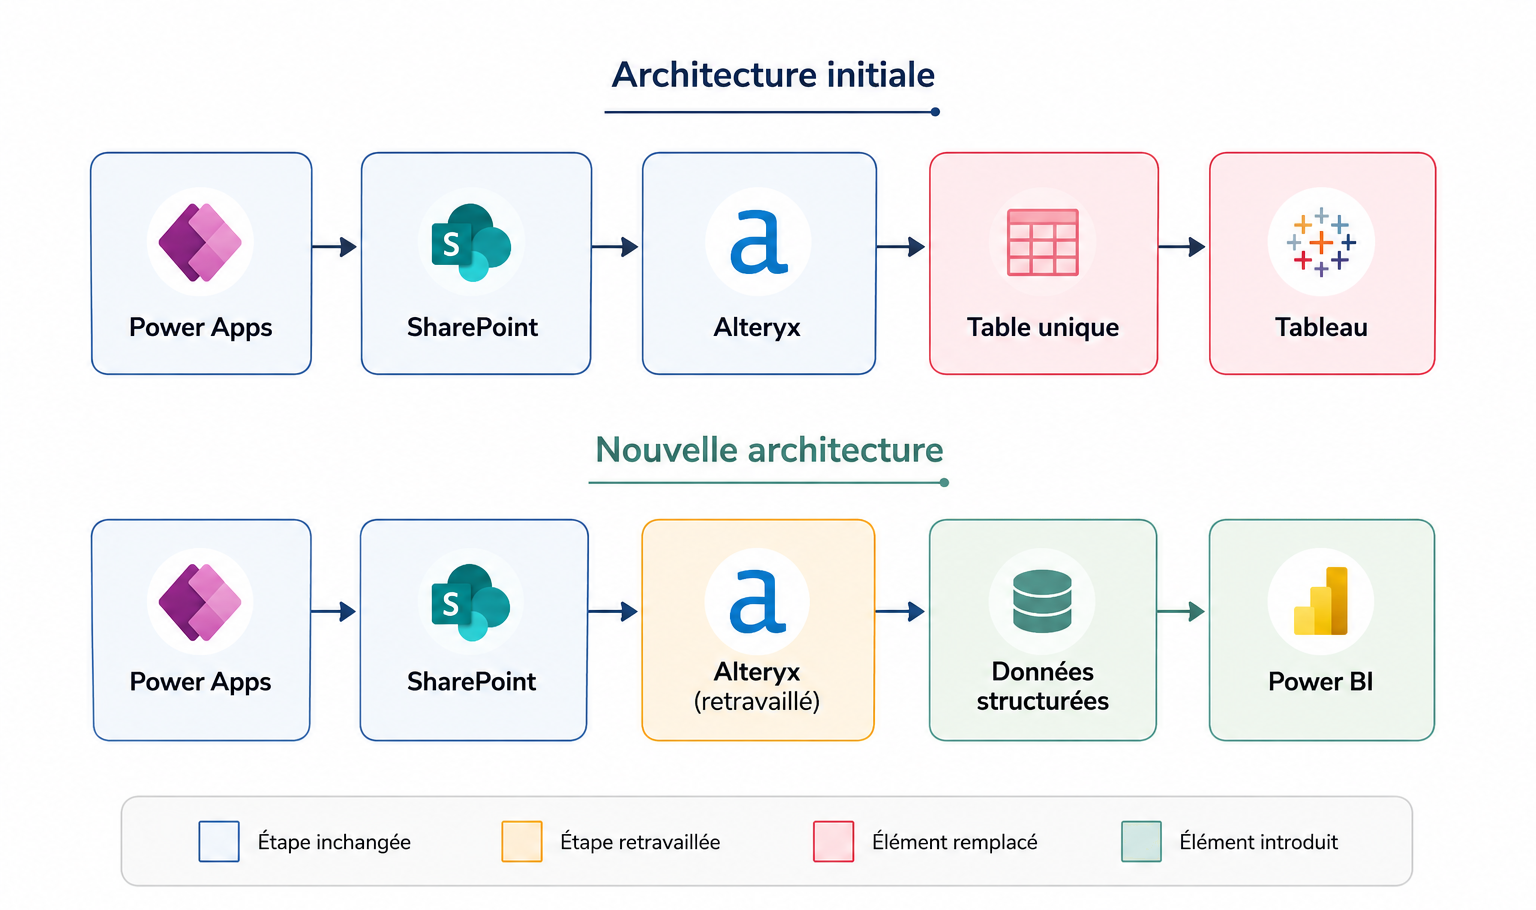
\includegraphics[draft=false,width=\textwidth]{cover/figures/archii_avant_apres.png}
\end{tcolorbox}
\caption{Évolution synthétique de la chaîne Data et décisionnelle d'IPANEMA}
\label{fig:evolution-architecture-ipanema}
\end{figure}

Le changement réalisé ne se résume donc pas au remplacement de Tableau par Power 
BI. Il repose également sur une refonte de la manière dont les données sont préparées et 
organisées avant leur restitution. Les choix de modélisation, les traitements réalisés et les 
aspects techniques de cette architecture seront développés dans le rapport d'étude.

\section{Réalisations et résultats obtenus}

Sur la base de cette réponse technique, les travaux ont été conduits jusqu'à leur terme 
selon la démarche itérative présentée en 1.5. À la date de rédaction de ce mémoire, le 
développement de la nouvelle solution est arrivé à son terme sur le plan fonctionnel et 
technique, la solution étant fonctionnelle de bout en bout. Mon intervention a couvert l'analyse 
de la chaîne existante, l'identification de ses limites, la restructuration des traitements de 
données, la construction du nouveau modèle, le développement des indicateurs et la 
réalisation du dashboard Power BI.

Ces travaux ont permis de faire évoluer IPANEMA d'une logique reposant sur une table 
unique vers une organisation structurée selon les différents niveaux de détail des données. La 
préparation, la structuration, les calculs et la restitution sont désormais davantage distingués, 
ce qui vise à rendre la chaîne plus compréhensible et plus facilement maintenable.

Le projet aboutit également à un nouveau dashboard développé sous Power BI, permettant d'inscrire le reporting IPANEMA dans l'environnement décisionnel cible. La solution 
obtenue répond ainsi à la fois à l'enjeu initial de fiabilisation de la donnée et à l'objectif de 
migration technologique.

\begin{table}[h!]
\centering
\caption{Comparaison avant/après le projet IPANEMA}
\label{tab:avant-apres-ipanema}
\vspace{6pt}
\renewcommand{\arraystretch}{1.5} % Augmente l'espace haut/bas dans les cellules
\setlength{\tabcolsep}{10pt}     % Augmente l'espace gauche/droite
\begin{tabular}{|>{\raggedright\arraybackslash}p{5cm}|>{\raggedright\arraybackslash}p{8.5cm}|}
\hline
\textbf{Avant le projet} & \textbf{À l'issue du développement} \\
\hline
Consolidation dans une table unique & Données organisées selon leurs différents niveaux de détail \\
\hline
Jointures pouvant générer des duplications ou pertes d'enregistrements & Restructuration des traitements afin de limiter ces situations \\
\hline
Reporting sous Tableau & Nouveau reporting développé sous Power BI \\
\hline
Chaîne complexe à faire évoluer & Séparation plus claire des différentes étapes de traitement \\
\hline
Contrôle principalement sur le résultat final & Tests et ajustements progressifs au cours du développement \\
\hline
\end{tabular}
\end{table}

La validation n'a pas été reportée à la seule fin du projet. Des tests et des revues ont 
été réalisés progressivement pendant le développement avec l'interlocuteur métier impliqué 
dans son suivi. Ces échanges ont permis de confronter régulièrement les réalisations au 
besoin, d'identifier les écarts et d'apporter les ajustements nécessaires. Les retours obtenus à 
ce stade sont favorables et confortent les orientations retenues.

La dernière étape avant la mise en production reste néanmoins la recette fonctionnelle 
élargie aux différents utilisateurs d'IPANEMA. Son organisation a été décalée en raison de 
contraintes de calendrier et de disponibilité des parties prenantes, notamment pendant la 
période estivale. 

Cette recette sera organisée sous la forme de demi-journées d'ateliers dédiés. Des 
scénarios représentatifs des usages d'IPANEMA seront définis puis exécutés avec les 
différents profils utilisateurs afin de vérifier la cohérence des données, la conformité des 
indicateurs et l'adéquation du dashboard avec les usages métier. Les retours recueillis 
permettront de distinguer les éventuelles anomalies devant être corrigées avant la mise en 
production des demandes d'amélioration susceptibles d'alimenter une évolution ultérieure de 
la solution. 

À ce stade, le bilan doit donc être nuancé : les objectifs liés à la restructuration de la 
chaîne Data et au développement sous Power BI sont atteints sur le plan de la réalisation, 
tandis que la validation définitive de certains critères fonctionnels reste conditionnée aux 
ateliers de recette. Cette distinction permet de ne pas considérer comme définitivement validés 
des résultats qui doivent encore être confrontés à l'ensemble des utilisateurs. 

\section{Principaux éléments de management du projet}

Le projet IPANEMA a été conduit selon une démarche agile adaptée au fonctionnement 
de l'équipe, fondée sur des cycles courts de réalisation, de validation et d'ajustement. Sans 
appliquer strictement un framework tel que Scrum, l'organisation retenue privilégie la 
collaboration, le feedback régulier et la capacité à adapter les travaux aux constats effectués 
au cours du projet.

Le pilotage s'appuie sur un suivi visuel des activités inspiré du Kanban, complété par 
des cartes mentales évolutives permettant de structurer les travaux et de capitaliser 
progressivement les informations nécessaires à leur documentation. Des points réguliers avec 
mon maître d'apprentissage permettent de partager l'avancement, de valider les orientations 
et de définir les prochaines étapes. Entre ces échanges, je conduis mes travaux de manière autonome et sollicite directement les personnes concernées lorsqu'un blocage nécessite un 
échange ou un arbitrage. 

La démarche peut ainsi être synthétisée par la boucle suivante :

\begin{center}
\begin{tcolorbox}[
    colframe=gray!60,       % Bordure gris doux
    colback=gray!4!white,   % Fond très clair
    boxrule=0.8pt,          % Épaisseur du cadre
    arc=5pt,                % Coins légèrement arrondis
    width=\textwidth,       % S'adapte à la largeur du texte
    halign=center,          % Centrage parfait du contenu
    top=8pt, bottom=8pt
]
\small\bfseries
Planifier 
\;\textcolor{gray!80}{$\longrightarrow$}\; 
Réaliser 
\;\textcolor{gray!80}{$\longrightarrow$}\; 
Tester 
\;\textcolor{gray!80}{$\longrightarrow$}\; 
Recueillir les retours 
\;\textcolor{gray!80}{$\longrightarrow$}\; 
Ajuster
\end{tcolorbox}
\end{center}


Cette logique s'est concrétisée par les validations progressives réalisées pendant le 
développement et se poursuivra lors des ateliers de recette. Elle permet de faire évoluer la 
solution en fonction des constats et des retours métier plutôt que d'attendre la fin du projet 
pour confronter le résultat aux besoins des utilisateurs. 

Cette présentation est volontairement synthétique. L'organisation des tâches, le 
schéma heuristique, les outils de pilotage, le planning prévisionnel et réalisé, l'analyse des 
écarts ainsi que les relations avec le maître d'apprentissage et l'équipe projet seront 
développés dans la partie spécifiquement consacrée au management du projet, conformément 
aux attendus de l'école.


\section{ Conclusion}
\label{sec16}
%=====================================%
Le projet IPANEMA a dépassé l'objectif initial d'une simple migration du reporting de 
Tableau vers Power BI. L'analyse de l'existant a mis en évidence la nécessité d'intervenir en 
amont de la visualisation afin de repenser la structuration des données et de fiabiliser leur 
exploitation. Le projet a ainsi abouti à une nouvelle chaîne Data structurée et à un nouveau 
dashboard Power BI destiné aux équipes Qualité. 

À ce stade, la réalisation technique est aboutie et la solution, fonctionnelle de bout en bout, a 
fait l'objet de validations progressives tout au long de son développement. Les ateliers de 
recette permettront désormais d'élargir cette validation aux différents utilisateurs avant la mise 
en production et, le cas échéant, d'identifier des améliorations pour une version ultérieure. Le 
rapport d'étude développera les analyses et les choix techniques ayant conduit à cette 
solution.

\chapter{ RAPPORT D’ÉTUDE : Refonte de la chaîne de traitement et de valorisation des données d’IPANEMA }
\minitoc
\label{chap2}
\newpage

%=====================================%
\section{Introduction}
\label{sec21}
%---------------------------------------------------------%
Le rapport d'action a présenté une synthèse du projet IPANEMA et de ses résultats. Ce rapport 
d'étude revient plus en détail sur la démarche suivie : l'analyse du besoin métier, le diagnostic 
de l'architecture existante, la formalisation des exigences, puis la conception de la nouvelle 
architecture Data et décisionnelle. 

%=====================================% 
\section{ Contexte et problématique}
\label{sec:sec22}
%=====================================% 
\subsection{ IPANEMA et la maîtrise des Tierces Parties }
IPANEMA, acronyme de International Partners Network & Management, est une solution 
informatique utilisée au sein de la R&D Dermo-Cosmétique & Personal Care (DC&PC) de 
Pierre Fabre pour accompagner le processus de maîtrise des Tierces Parties. Dans ce 
contexte, une Tierce Partie désigne une entité extérieure au groupe dont l’activité peut avoir 
un impact direct ou indirect sur la qualité d’un produit ou sur la sécurité du patient, du 
consommateur ou du client.

La collaboration avec ces acteurs implique donc un suivi permettant d’identifier et 
d’évaluer les risques associés à leurs activités. IPANEMA intervient comme support 
numérique de ce processus : l’application centralise les informations nécessaires à l’évaluation 
des Tierces Parties et permet aux différents acteurs concernés de participer à leur suivi.

Les informations collectées ne constituent cependant qu’une première étape. Pour 
qu’elles puissent réellement contribuer au pilotage de l’activité, elles doivent être transformées 
en informations fiables, compréhensibles et exploitables par les équipes Qualité. Le reporting 
occupe ainsi une place importante dans la chaîne de valeur d’IPANEMA : il constitue le point 
de rencontre entre les données produites par le processus d’évaluation et leur utilisation à des 
fins de suivi et de prise de décision.

Cette dimension est au cœur du projet présenté dans ce rapport. 

\begin{figure}[H]
    \centering
    \fbox{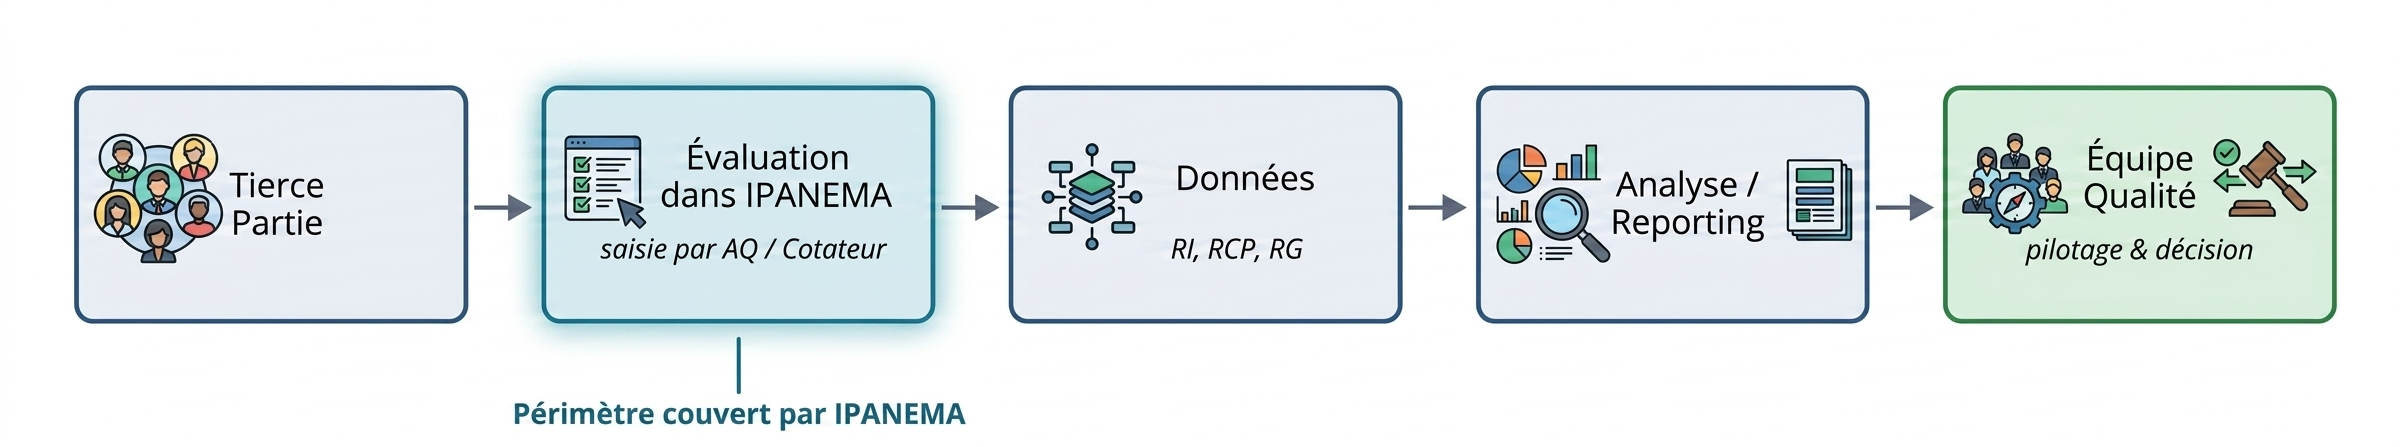
\includegraphics[width=5.5cm]{cover/figures/processusde_maîtrise_des_Tierces.jpg}}
    \caption{Positionnement d’IPANEMA dans le processus de maîtrise des Tierces Parties.}
    \label{fig:processusde_maîtrise_des_Tierces}
\end{figure}

%=====================================%    

\subsection{ Périmètre du projet IPANEMA V2  }\label{subsec:Perimètre du projet IPANEMA V2} 

Dans le cadre de son évolution, IPANEMA a fait l’objet d’une refonte vers une seconde 
version. Le projet global a été organisé autour de deux périmètres complémentaires. 

La Partie A concerne l’évolution de l’application métier développée sous Power Apps. 
Cette partie, confiée à un prestataire externe, comprend notamment la refonte des interfaces 
d’administration et de cotation, l’évolution de certaines fonctionnalités ainsi que la migration 
des données historiques. 

La Partie B concerne quant à elle la valorisation des données générées par IPANEMA. 
Elle comprend l’adaptation de la chaîne de traitement, l’intégration des calculs associés aux 
risques la mise à jour des indicateurs et la refonte du reporting. C’est sur ce second périmètre 
que s’inscrit mon projet d’alternance. 

Mon intervention ne s'est donc pas limitée à reproduire sous Power BI les visualisations 
historiquement disponibles sous Tableau. Les anomalies identifiées dans l'existant ont 
nécessité de réexaminer la manière dont les données étaient préparées, regroupées et mises 
en relation avant leur restitution. Le projet comporte ainsi deux dimensions étroitement liées : 
une dimension Data, portant sur la préparation, la structuration, la modélisation et la 
fiabilisation des données, et une dimension Business Intelligence, consacrée à la construction 
des indicateurs et à leur restitution dans un outil de pilotage adapté aux besoins des équipes 
Qualité. 

\begin{figure}[H]
    \centering
    \fbox{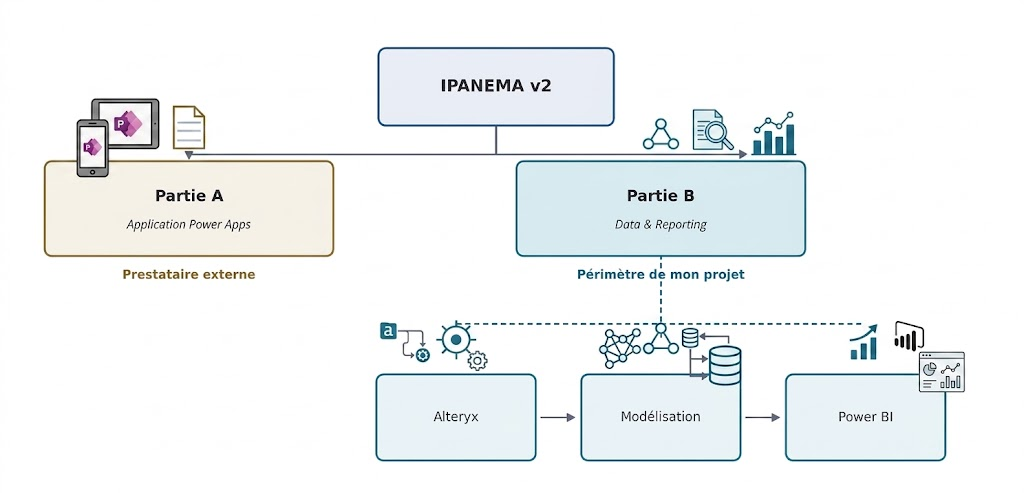
\includegraphics[width=5.5cm]{cover/figures/Périmètre_du_projet_IPANEMA_v2.jpg}}
    \caption{Périmètre du projet IPANEMA v2 : répartition entre la Partie A (application Power Apps, prestataire externe) et la Partie B (Data & Reporting, périmètre de mon projet).}
    \label{fig:Perimètre_du_projet_IPANEMA_v2}
\end{figure}


%=====================================%\n
\subsection{Problématique de l’étude}
%---------------------------------------------------------%
La première version du reporting IPANEMA reposait sur une chaîne associant Power Apps, SharePoint, Alteryx et Tableau. Les données saisies par les utilisateurs étaient stockées dans différentes listes SharePoint, puis consolidées au moyen de traitements Alteryx avant 
d’être restituées dans un dashboard Tableau. À l’usage, plusieurs limites ont été identifiées. La consolidation de données possédant 
des granularités différentes dans une table unique pouvait entraîner des duplications ou, selon 
les jointures réalisées, la disparition de certains enregistrements. Ces phénomènes étaient 
susceptibles d’affecter directement les indicateurs présentés aux utilisateurs. Des difficultés 
relatives à la maintenance, aux performances et à la lisibilité de la restitution ont également 
été remontées. 

Dans le même temps, l’environnement décisionnel du groupe évoluait progressivement 
vers l’écosystème Microsoft et Power BI. La migration constituait donc une opportunité pour 
ne pas simplement remplacer l’outil de visualisation, mais repenser plus globalement la chaîne 
de valorisation des données d’IPANEMA.

La problématique retenue pour cette étude est ainsi la suivante :

\textbf{Comment repenser la structuration et la restitution des données d’IPANEMA afin de fiabiliser le suivi des Tierces Parties, tout en proposant aux équipes Qualité un outil de pilotage performant, maintenable et intégré à l’écosystème Microsoft du groupe ?}
\\
La réponse à cette problématique nécessite d’abord de comprendre le processus métier 
à l’origine des données.

\section{Compréhension du besoin métier}

\subsection{Les acteurs et utilisateurs d’IPANEMA}

IPANEMA intervient dans un processus impliquant plusieurs catégories d’utilisateurs, 
dont les responsabilités et les besoins diffèrent. Quatre profils principaux sont identifiés dans 
l’application : \textbf{ Administrateur, Assurance Qualité (AQ), Cotateur et Consultation.}

L’\textbf{Administrateur} assure notamment la gestion des utilisateurs et de leurs droits d’accès. 
Son intervention garantit que chaque utilisateur dispose des fonctionnalités correspondant à 
son rôle. 

Le profil \textbf{Assurance Qualité} occupe une place centrale dans le processus. Il intervient 
dans le pilotage des Tierces Parties et des campagnes d’évaluation, dans la configuration de 
certains paramètres nécessaires à l’évaluation ainsi que dans la validation des informations 
renseignées. 

Le \textbf{Cotateur} appartient aux équipes métier en relation avec la Tierce Partie. Il intervient 
directement dans le processus d’évaluation en renseignant les critères qui relèvent de son 
périmètre. 

Enfin, le profil \text{Consultation} dispose d’un accès en lecture aux informations et 
évaluations finalisées, sans possibilité de modification. 

Cette diversité de profils implique que les données produites par IPANEMA ne répondent 
pas uniquement à une logique de stockage. Elles représentent le résultat d’un processus 
collaboratif, au cours duquel plusieurs acteurs interviennent successivement sur une même évaluation. Cette caractéristique aura une incidence directe sur la manière dont les données 
devront être modélisées, comme le montre la partie suivante.

\begin{figure}[H]
    \centering
    \fbox{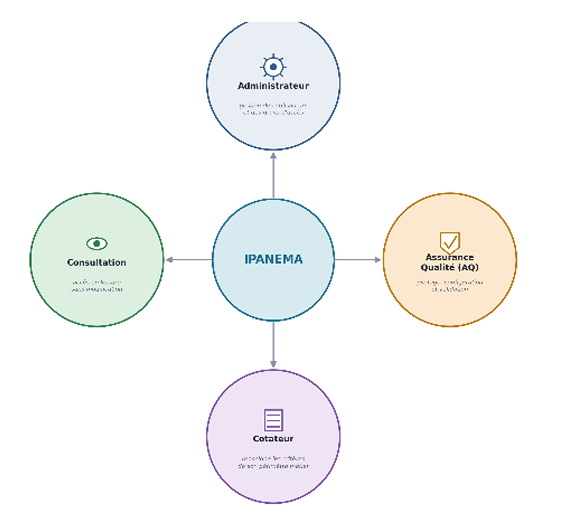
\includegraphics[width=0.25\textwidth]{cover/figures/quatre_profils_d'utilisateurs.png}}
    \caption{Les quatre profils d'utilisateurs d'IPANEMA et leur rôle dans le processus d'évaluation des Tierces Parties.}
    \label{fig:quatre_profils_d'utilisateurs}
\end{figure}


\subsection{Processus d’évaluation d’une Tierce Partie }

L’évaluation d’une Tierce Partie est réalisée dans le cadre d’une campagne. Une grille 
d’évaluation est générée, puis renseignée successivement par les acteurs concernés. 

Le Cotateur commence par compléter les critères correspondant à son périmètre 
métier. Une fois cette étape terminée, l’évaluation est transmise à l’Assurance Qualité, qui 
complète à son tour les éléments relevant de son domaine de responsabilité. L’AQ peut 
ensuite valider l’évaluation ou la retourner au Cotateur lorsqu’une correction ou un 
complément est nécessaire. Les changements de statut permettent ainsi de suivre la 
progression de l’évaluation jusqu’à sa finalisation.  

Ce fonctionnement est important d’un point de vue Data. Une Tierce Partie peut être 
associée à plusieurs campagnes et plusieurs évaluations au cours du temps. Une évaluation 
comporte elle-même plusieurs critères. Ces différents niveaux d’information ne possèdent 
donc pas nécessairement la même granularité : une donnée décrivant une Tierce Partie n’a 
pas le même niveau de détail qu’une donnée décrivant une campagne, une évaluation ou un 
critère. Leur rapprochement doit donc respecter les relations qui existent entre ces objets 
métier. Cette notion constitue l'un des points structurants du projet, et sera au cœur du 
diagnostic présenté en 2.3. 

\begin{figure}[H]
    \centering
    \fbox{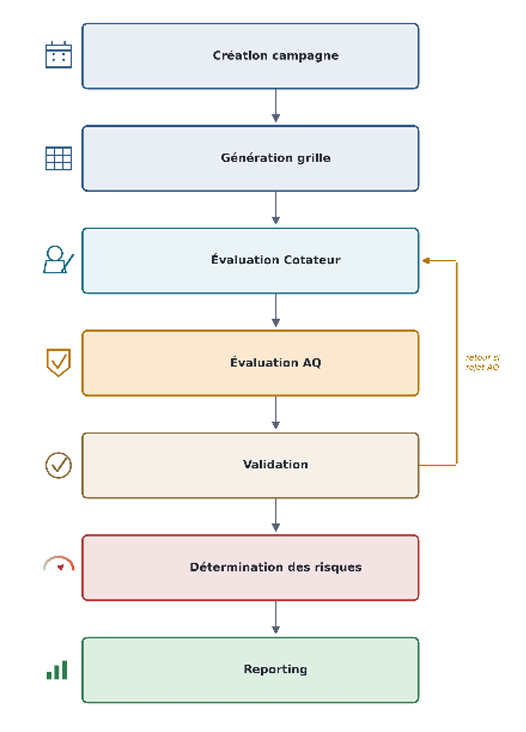
\includegraphics[width=0.25\textwidth]{cover/figures/processus_evaluation_tierce_partie.png}}
    \caption{Processus d'évaluation d'une Tierce Partie, de la création de la campagne au reporting. }
    \label{processus_evaluation_tierce_partie}
\end{figure}

\subsection{Les niveaux de risque}

Le processus d'évaluation repose sur trois notions de risque, dont le calcul constitue l'une 
des évolutions attendues de la solution cible : \textbf{le Risque Intrinsèque (RI), le Risque Conformité et Performance (RCP), et le Risque Global (RG)} qui en résulte.
\textbf{Le Risque Intrinsèque} caractérise le profil de risque propre à une Tierce Partie, 
indépendamment de la qualité de son exécution. Il est évalué annuellement par un utilisateur 
du profil AQ, à partir de sept critères portant sur des caractéristiques structurelles de la Tierce 
Partie : sa criticité, son niveau d'expertise et de savoir-faire, la complexité de la prestation (y 
compris en cas de sous-traitance en cascade), le référentiel qualité opposable, sa certification 
qualité et le volume de prestations attendu. Chaque critère est noté selon le niveau constaté, 
puis pondéré par un facteur qui varie selon que la Tierce Partie relève ou non du statut CDMO 
(\textbf{C}ontract \textbf{D}evelopment and \textbf{M}anufacturing \textbf{O}rganization). La somme des scores obtenus est 
ensuite comparée à la somme des scores maximum théoriquement atteignables, ce qui 
permet de classer le RI selon trois niveaux : LOW, MEDIUM, HIGH au moyen de seuils 
exprimés en fraction du score maximum.\\

\textbf{Le Risque Conformité et Performance} évalue, quant à lui, la manière dont la Tierce 
Partie exécute effectivement ses prestations. Il combine deux volets évalués par des profils 
distincts : un volet "Qualité", renseigné par l'AQ à partir des résultats d'audit et de la conformité 
qualité de la prestation, et un volet "Métier", renseigné par le Cotateur à partir de critères 
opérationnels tels que la qualité des livrables, la traçabilité, le respect des délais, le relationnel, 
les compétences techniques et la capacité d'innovation. Le score global obtenu est classé 
selon la même logique de seuils que pour le RI. Une particularité du RCP est qu'il n'est calculé 
que lorsque l'ensemble des évaluations de la Tierce Partie sur la campagne sont clôturées ; 
lorsqu'une Tierce Partie fait l'objet de plusieurs évaluations, le RCP retenu correspond à leur 
moyenne — une règle qui a une incidence directe sur la conception de la chaîne de données, 
puisqu'elle impose de disposer, avant le calcul, du statut de clôture de chaque évaluation 
associée.\\

\textbf{Le Risque Global} ne résulte pas d'une moyenne entre RI et RCP, mais d'une 
combinaison matricielle des deux niveaux. Cette logique traduit une approche volontairement 
conservatrice : une Tierce Partie présentant un RI élevé conserve un RG élevé même si son 
RCP est satisfaisant, ce qui reflète le fait que le risque intrinsèque (lié à la nature même de 
l'activité sous-traitée) ne peut être compensé par une bonne performance d'exécution. 
\\
Cette architecture de calcul, à trois niveaux imbriqués, a directement structuré la 
conception du modèle de données : elle impose de conserver la traçabilité des critères, des 
notes et des pondérations par campagne (ces paramètres pouvant évoluer d'une campagne 
à l'autre) et de restituer non seulement le RG final mais aussi les niveaux intermédiaires RI et 
RCP qui le composent. C'est précisément cette exigence d'historisation et de granularité qui 
rendait la logique de table unique inadaptée, comme le montre le diagnostic qui suit. 

\section{Analyse de l’existant et diagnostic}
\subsection{Architecture initiale}
Avant la refonte, les informations utilisées par IPANEMA provenaient principalement des 
deux applications Power Apps IPANEMA-Admin et IPANEMA-Cotation. Les données saisies 
étaient réparties dans 19 listes SharePoint.\\

Ces listes constituaient les différentes sources nécessaires à la restitution. Des workflows 
Alteryx permettaient de récupérer et de transformer les informations issues de SharePoint, 
auxquelles venaient également s’ajouter certaines données provenant de Trackwise. Les 
différentes sources étaient ensuite rapprochées afin de construire une table finale unique 
utilisée par Tableau.  

L’architecture pouvait ainsi être représentée de la manière suivante : 

\begin{center}
\begin{tcolorbox}[
    colframe=gray!60,       % Bordure gris doux
    colback=gray!4!white,   % Fond très clair
    boxrule=0.8pt,          % Épaisseur du cadre
    arc=5pt,                % Coins légèrement arrondis
    width=\textwidth,       % S'adapte à la largeur du texte
    halign=center,          % Centrage parfait du contenu
    top=8pt, bottom=8pt
]
\small\bfseries
Power Apps 
\;\textcolor{gray!80}{$\longrightarrow$}\; 
19 listes SharePoint 
\;\textcolor{gray!80}{$\longrightarrow$}\; 
Alteryx 
\;\textcolor{gray!80}{$\longrightarrow$}\; 
Table à plat 
\;\textcolor{gray!80}{$\longrightarrow$}\; 
Tableau
\end{tcolorbox}
\end{center}

Cette architecture avait l’avantage de fournir à l’outil de restitution un jeu de données 
directement exploitable. Cependant, la concentration de données de natures et de 
granularités différentes dans une même table a progressivement montré ses limites. 

\begin{figure}[H]
    \centering
    \fbox{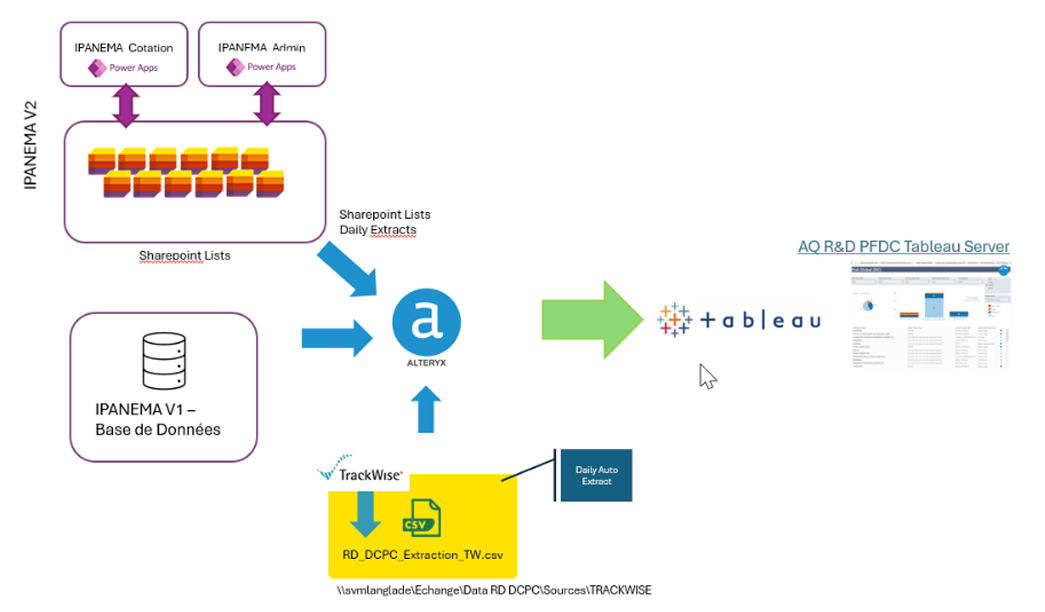
\includegraphics[width=0.25\textwidth]{cover/figures/Architecture_initiale_d'IPANEMA.png}}
    \caption{Architecture initiale d'IPANEMA : des sources de données jusqu'à la restitution de l'équipe Qualité (AQ R&D DCPC).}
    \label{Architecture_initiale_d'IPANEMA}
\end{figure}

\subsection{Analyse du traitement initial }
Le rôle d'Alteryx dans l'architecture initiale consistait à assurer les opérations d'extraction, 
de transformation et de préparation nécessaires avant la restitution des données. La difficulté 
ne résidait cependant pas dans l'utilisation d'Alteryx en elle-même, mais dans la logique de 
consolidation retenue : les informations issues des différentes sources étaient 
progressivement rapprochées au moyen de jointures successives, chaque nouvelle liste 
SharePoint étant intégrée à la table en cours de construction. Le schéma suivant illustre ce 
principe de manière simplifiée.  

\begin{figure}[H]
    \centering
    \fbox{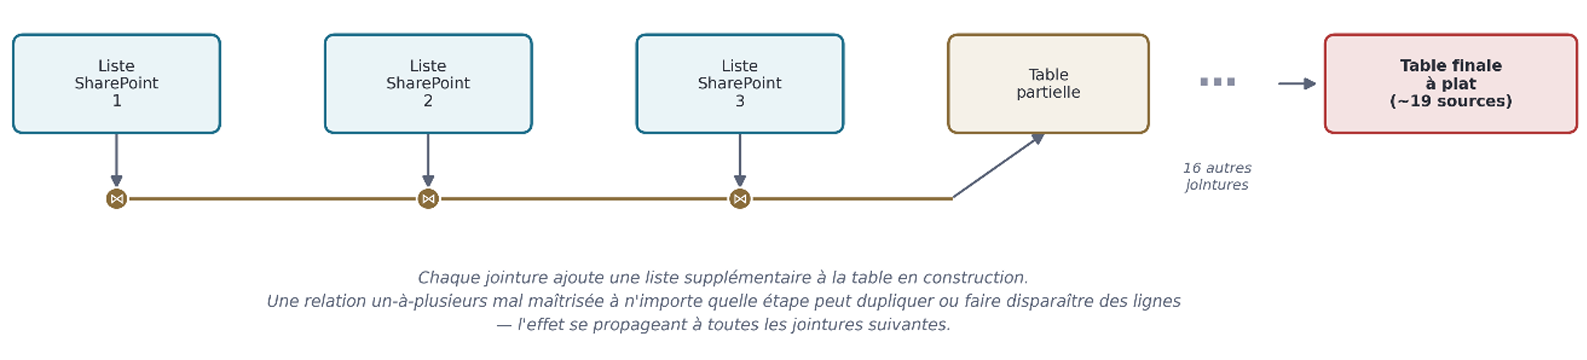
\includegraphics[width=0.25\textwidth]{cover/figures/jointures_successives_des_listes.png}}
    \caption{Principe de construction de l'ancienne table à plat : jointures successives des listes SharePoint en cascade.}
    \label{jointures_successives_des_listes}
\end{figure}

Ce principe, bien que simple dans sa logique, se traduisait dans la pratique par un 
enchaînement d'une vingtaine de jointures successives, correspondant chacune à l'intégration 
d'une nouvelle liste SharePoint. Le workflow réel, nettement plus dense que sa représentation 
schématique, donne une idée concrète de la complexité opérationnelle qui en résultait — 
complexité qui constitue en elle-même l'un des facteurs à l'origine des limites identifiées plus 
loin dans ce chapitre.

\begin{figure}[H]
    \centering
    \fbox{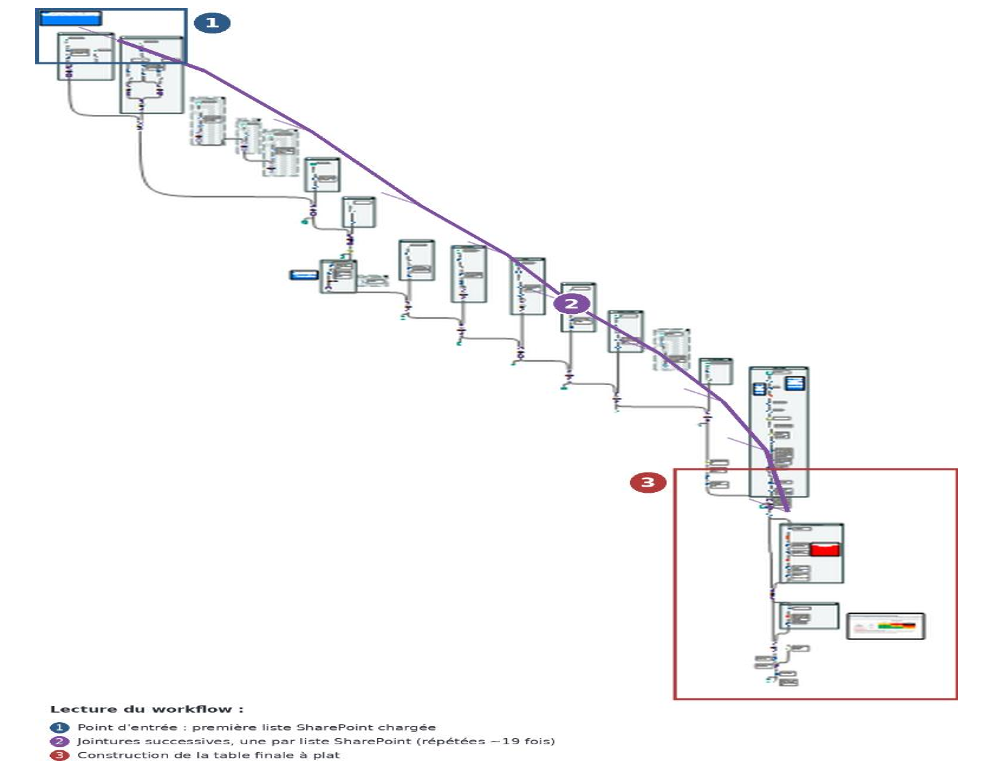
\includegraphics[width=0.25\textwidth]{cover/figures/Ancien_workflow_alteryx.png}}
    \caption{Ancien workflow Alteryx.}
    \label{Ancien_workflow_alteryx}
\end{figure}

Cette densité illustre un premier constat : au-delà des anomalies ponctuelles qu'elle a 
pu produire, cette architecture représentait déjà, par sa seule structure, un défi de 
maintenabilité. Mais la conséquence la plus directe de cette logique de jointures en cascade 
concerne la donnée elle-même. Les objets métier manipulés n'étaient en effet pas tous définis 
au même niveau de détail : une Tierce Partie peut, par exemple, être associée à plusieurs 
évaluations. Si les informations décrivant la Tierce Partie sont fusionnées directement avec 
celles décrivant chacune de ses évaluations, les données de la Tierce Partie sont 
nécessairement répétées pour chaque évaluation correspondante. Cette répétition n'est pas 
problématique en elle-même, elle le devient lorsque la table résultante est utilisée pour 
effectuer des comptages ou des agrégations sans tenir compte de cette granularité. \\

Cette architecture en cascade a ainsi une conséquence structurelle importante : une 
relation un-à-plusieurs mal maîtrisée à n'importe quelle étape de l'enchaînement se propage 
à l'ensemble des jointures suivantes, amplifiant mécaniquement le risque de duplication ou de 
perte d'enregistrements à mesure que le nombre de sources intégrées augmente. C'est 
précisément ce phénomène qui est détaillé dans le diagnostic ci-après. 

\subsection{Limites et anomalies identifiées}

L’analyse de l’existant, menée notamment lors des échanges avec le développeur du 
dashboard Tableau, mon maître d’apprentissage et les équipes Qualité, a permis de mettre 
en évidence plusieurs catégories de limites.

\textbf{a) Duplication des données}\\
La première difficulté concernait la duplication de certains enregistrements. Lorsqu’une 
relation de type un-à-plusieurs était intégrée dans la table unique, une même information 
pouvait être répétée sur plusieurs lignes. \\
Ces duplications pouvaient avoir une incidence directe sur certains indicateurs. Un 
comptage réalisé sans tenir compte de la granularité réelle des données risquait alors de 
comptabiliser plusieurs fois un même objet métier.

\text{b) Disparition de certains enregistrements}\\
Le phénomène inverse pouvait également se produire. Selon le type de jointure et la 
disponibilité des clés utilisées pour rapprocher les sources, certains enregistrements pouvaient 
ne pas être conservés dans le jeu de données final. \\
Une Tierce Partie présente dans une source pouvait ainsi ne plus apparaître dans le 
dashboard lorsque les conditions nécessaires à son rapprochement avec une autre table 
n’étaient pas satisfaites. 

\textbf{c) Valeurs manquantes interprétées à tort comme des notes. }\\
Ce point constitue l'une des anomalies les plus critiques identifiées, car elle ne produisait 
pas une simple erreur visible, mais une fausse donnée silencieuse : un résultat en apparence 
cohérent, mais construit sur une base erronée. Le mécanisme se déroule en plusieurs étapes. 
D'abord, comme détaillé en 2.3.2, la logique de jointures en cascade pouvait dupliquer certains 
enregistrements lorsqu'une relation un-à-plusieurs était mal maîtrisée. Parmi ces lignes 
dupliquées, certaines correspondaient à des critères ou des évaluations pour lesquels aucune 
note n'avait réellement été attribuée par l'utilisateur : l'évaluation était simplement absente, 
non renseignée. Le traitement existant, plutôt que de conserver cette absence de valeur telle 
quelle, la remplaçait automatiquement par 0. \\
C'est à ce stade que le problème devient critique : dans la logique de notation du RI et 
du RCP (cf. 2.2.3), 0 n'est pas une valeur neutre mais c'est la meilleure note possible, celle 
correspondant au niveau de risque le plus favorable. Une case vide, remplie automatiquement 
par 0, n'était donc pas traitée comme "pas d'information disponible", mais comme "cette Tierce 
Partie a été évaluée, et elle a obtenu la meilleure note sur ce critère". Une Tierce Partie qui 
n'avait tout simplement pas été évaluée sur un critère donné se retrouvait ainsi, après 
traitement, avec un score identique à celui d'une Tierce Partie réellement évaluée et jugée 
sans aucun risque sur ce critère. Le système ne pouvait plus distinguer ces deux situations 
pourtant radicalement différentes « on ne sait pas » et « on sait, et c'est excellent » produisant 
exactement le même résultat chiffré. Cette confusion faussait mécaniquement à la baisse les 
scores globaux RI et RCP des Tierces Parties concernées, pouvant les faire apparaître comme 
moins risquées qu'elles ne l'étaient réellement, un biais d'autant plus dangereux qu'il restait 
invisible sans investigation approfondie. \\

À cette confusion s'ajoutaient deux anomalies connexes, également liées au traitement 
des données absentes : certaines valeurs N/A remontaient dans certains cas jusque dans la 
restitution finale, sans traitement en amont, et certains enregistrements comportaient dans les 
données sources la valeur texte littérale "Null" plutôt qu'une valeur réellement vide : une 
nuance que les traitements existants ne géraient pas correctement, ce qui pouvait à son tour 
entraîner des duplications de lignes lors des jointures. Ce dernier cas a par exemple été 
identifié sur des partenaires dont l'activité est de type Development et le statut CDMO. 

\textbf{d) Complexité des calculs }\\
La restitution des risques RI, RCP et RG nécessite l’application de règles métier 
spécifiques. La structure de la table finale rendait certains traitements difficiles à maintenir et 
pouvait conduire à des résultats ne correspondant pas systématiquement aux valeurs 
attendues. 

\textbf{e) Maintenabilité }\\
La concentration d’une grande quantité d’informations dans une table unique augmentait 
également la complexité de maintenance. Toute évolution d’une source, d’une règle métier ou 
d’un indicateur pouvait nécessiter d’intervenir sur une chaîne de transformations comportant 
de nombreuses dépendances.\\

\textbf{Exemple concret} \\
L'écart observé sur l'indicateur de satisfaction "Innovation" du partenaire Cebiphar 
(campagne 2025) illustre concrètement l'impact de cette confusion entre absence d'évaluation 
et note favorable. Le dashboard Tableau affichait pour ce critère une valeur de 0,39, nettement 
inférieure aux autres critères de la même Tierce Partie, pourtant tous évalués de manière 
cohérente et satisfaisante. 

\begin{figure}[H]
    \centering
    \fbox{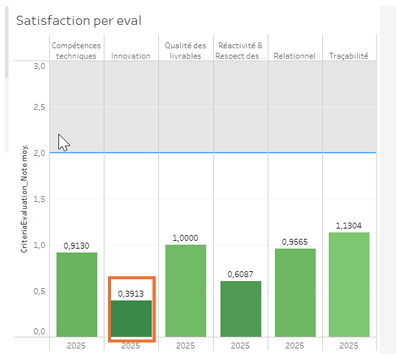
\includegraphics[width=0.1\textwidth]{cover/figures/valeur_anormalement_basse.png}}
    \caption{Ancien dashboard Tableau : satisfaction par critère pour Cebiphar (campagne 2025), avec une valeur anormalement basse sur le critère Innovation (0,39).}
    \label{valeur_anormalement_basse}
\end{figure}

L'analyse de cet écart a montré que le calcul Tableau intégrait, dans la moyenne du 
critère, les évaluations au statut "Not Evaluated", c'est-à-dire des évaluations non réalisées au 
même titre que les évaluations réellement renseignées. Cette confusion, décrite plus haut, 
faussait mécaniquement l'indicateur à la baisse.

Le nouveau dashboard Power BI, qui exclut correctement les statuts "Not Evaluated" du 
calcul, restitue pour ce même critère une valeur de 1,00 soit la note maximale, cohérente avec 
les autres critères de ce partenaire. 

\begin{figure}[H]
    \centering
    \fbox{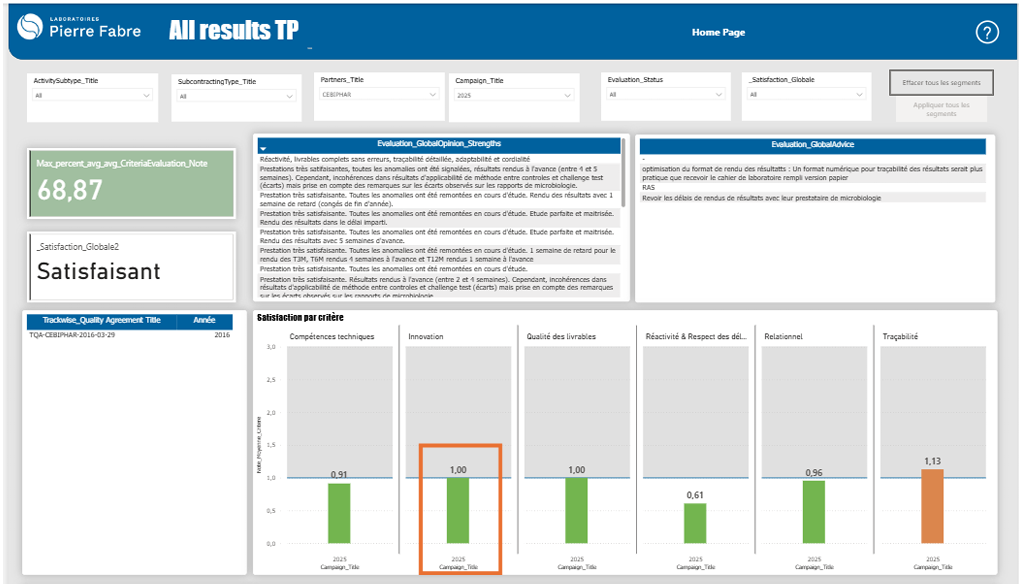
\includegraphics[width=0.1\textwidth]{cover/figures/Nouveau_dashboard_Power_BI.png}}
    \caption{Nouveau dashboard Power BI : satisfaction par critère pour Cebiphar (campagne 2025), avec une valeur corrigée de 1,00 sur le critère Innovation.}
    \label{Nouveau_dashboard_Power_BI}
\end{figure}

Cette correction a été vérifiée directement à la source, dans la liste SharePoint 
CriteriaEvaluation. En filtrant les évaluations sur le critère Innovation et en excluant les statuts 
"Not Evaluated", l'ensemble des notes réellement attribuées par les utilisateurs affiche une 
valeur de 1, confirmant que la valeur de 0,39 observée dans Tableau ne provenait pas d'une 
évaluation défavorable, mais bien de l'inclusion erronée d'évaluations non renseignées dans 
le calcul de la moyenne.

\begin{figure}[H]
    \centering
    \fbox{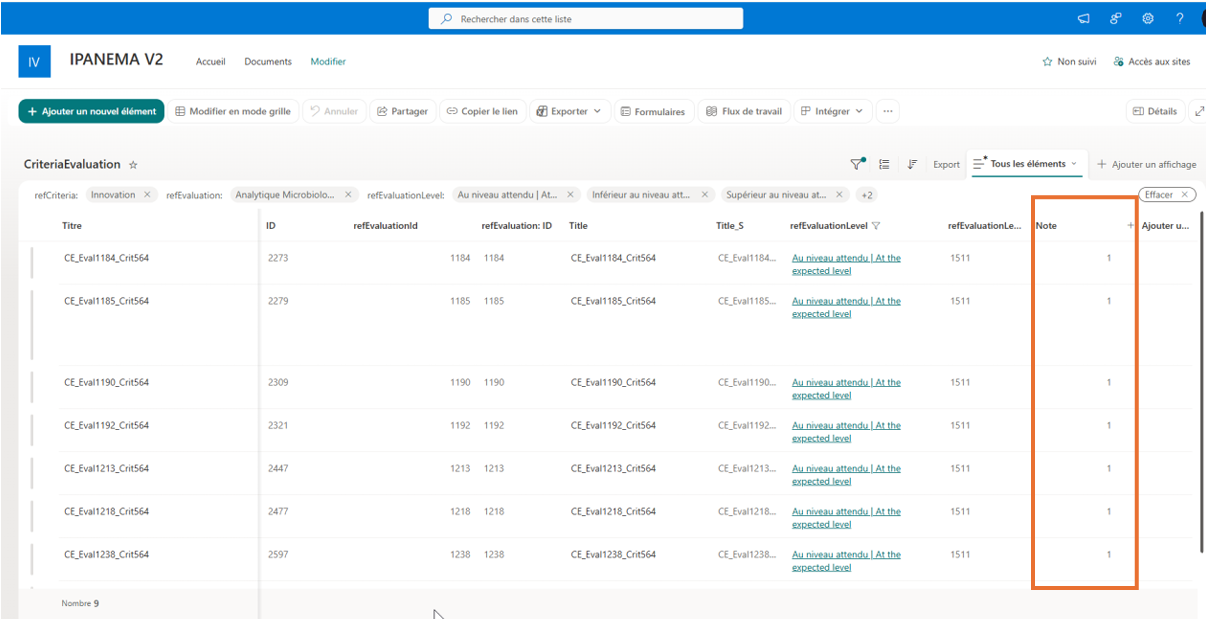
\includegraphics[width=0.1\textwidth]{cover/figures/Extrait_de_la_liste_SharePoint_CriteriaEvaluation.png}}
    \caption{Extrait de la liste SharePoint CriteriaEvaluation, filtré sur le critère Innovation : les notes effectivement attribuées valent toutes 1, confirmant la valeur restituée par Power BI.}
    \label{Extrait_de_la_liste_SharePoint_CriteriaEvaluation}
\end{figure}

La vérification à la source a par ailleurs révélé une difficulté supplémentaire : la colonne 
refEvaluationLevel de la table CriteriaEvaluation, censée permettre de distinguer les critères 
évalués des critères non évalués, comportait en réalité deux variantes distinctes du libellé "non 
évalué" (une différence de casse dans la traduction anglaise du libellé). Un filtre appliqué sur 
une seule de ces deux valeurs aurait donc laissé passer une partie des critères non évalués, 
faussant à nouveau le résultat. La vérification présentée en figure 11 a été réalisée en excluant 
systématiquement les deux variantes, afin de ne conserver que les critères réellement évalués 
illustrant, à une échelle plus fine encore, la même exigence de rigueur sur le traitement des 
données manquantes que celle décrite au point c).\\
Ce cas démontre, sur un exemple réel et vérifié à la source, la nécessité identifiée en 
amont : distinguer explicitement l'absence d'évaluation d'une évaluation réellement favorable, 
faute de quoi les indicateurs de risque et de performance perdent leur fiabilité avec un écart 
pouvant dépasser 0,6 point sur une échelle de 0 à 1, comme observé ici.

\subsection{Diagnostic}
L'analyse menée montre que les limites observées ne peuvent pas être attribuées à l'outil 
de visualisation seul : le dashboard Tableau restituait fidèlement les données qu'on lui 
transmettait, la défaillance se situant en amont, dans leur préparation.
\\
Trois causes s'en dégagent. Une cause architecturale : les jointures en cascade 
consolidaient des objets métier de granularités différentes dans une table unique, propice aux 
duplications et aux pertes d'enregistrements. Une cause sémantique : la confusion entre 
absence d'évaluation et note de 0 conduisait le système à traiter deux réalités opposées 
comme une seule donnée. Une cause liée à la gouvernance du référentiel : l'incohérence des 
valeurs de référence, comme le double libellé "non évalué", pouvait fausser les traitements en 
aval même lorsque leur logique était correcte.
\\
Le passage à Power BI ne pouvait donc pas se limiter à une migration à l'identique du 
dashboard existant : cela aurait déplacé l'interface de restitution sans corriger aucune de ces 
causes. La refonte devait intervenir à plusieurs niveaux : la préparation des données, pour 
limiter les effets en cascade des jointures ; la gestion explicite des valeurs manquantes ; 
l'organisation des données en entités cohérentes respectant leur granularité ; les relations 
entre ces entités, reconstruites au niveau du modèle plutôt qu'à plat ; le calcul des indicateurs 
RI, RCP et RG ; et leur restitution aux utilisateurs.
\\
Ce diagnostic constitue le point de départ de la solution proposée et structure la formalisation des exigences qui suit. 

\section{Formalisation du besoin et des exigences}
\subsection{Expression du besoin : Diagramme « bête à cornes »}
Afin de formaliser la finalité du projet indépendamment des choix technologiques, le 
besoin a été représenté à l’aide du diagramme « bête à cornes ». \\
Il permet de répondre à trois questions fondamentales : \\
\textbf{À qui le système rend-il service ?}
Aux équipes Qualité de la R&D DC&PC chargées du suivi des Tierces Parties. \\
\textbf{Sur quoi agit-il ?}
Sur les données issues de l’évaluation et du suivi des Tierces Parties. \\
\textbf{Dans quel but ? }
Fournir une information fiable et exploitable permettant de faciliter leur pilotage et la maîtrise 
des risques associés.

\begin{figure}[H]
    \centering
    \fbox{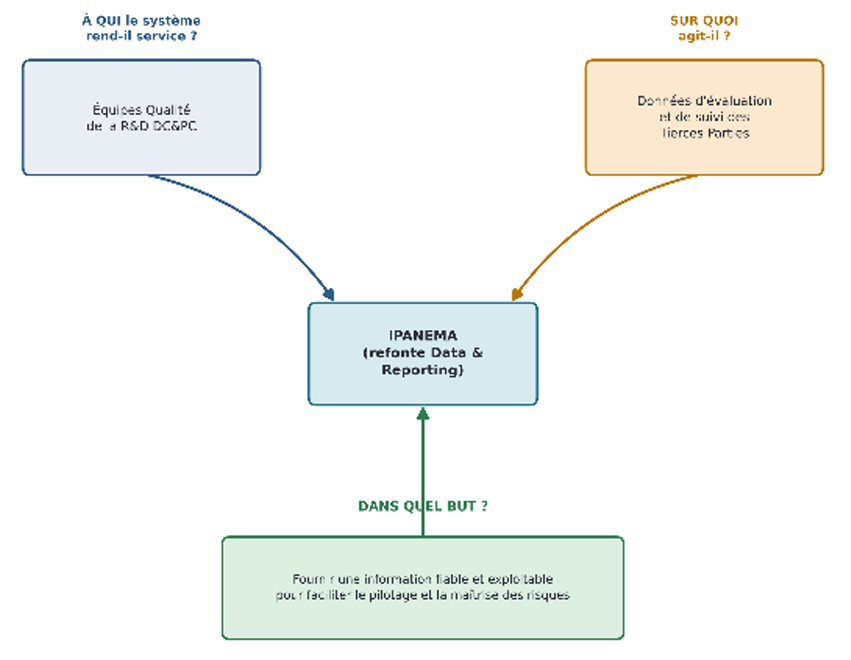
\includegraphics[width=0.1\textwidth]{cover/figures/Formalisation_du_besoin_du_projet_IPANEMA.png}}
    \caption{Formalisation du besoin du projet IPANEMA selon la méthode « bête à cornes »}
    \label{Formalisation_du_besoin_du_projet_IPANEMA}
\end{figure}

L’intérêt de cette représentation est de rappeler que la finalité du projet n’est pas la 
migration vers Power BI en elle-même. La technologie constitue un moyen permettant de 
répondre à un besoin métier : mettre à disposition des équipes Qualité une information fiable 
leur permettant de piloter les Tierces Parties.

\subsection{Besoins exprimés par les utilisateurs} 
Les attentes des équipes Qualité se sont précisées progressivement, au fil des 
réunions d'avancement et des retours sur les versions successives du dashboard. Six 
grandes catégories de besoins se dégagent, chacune distinguant ce qui a été exprimé par 
les utilisateurs de sa traduction technique.


%=====================================%
\section{Campagne de tests du premier module de la plateforme} 
%---------------------------------------------------------%

Dans la continuité de la phase de développement, une campagne de tests a été menée afin de valider la première version du module de recrutement des bénéficiaires de la plateforme RI2S. Cette étape avait pour objectif de garantir la conformité fonctionnelle et technique des premières fonctionnalités livrées, et d’évaluer la robustesse de la solution en vue d’une mise en production progressive.



\subsection{Objectif de la campagne}
Cette campagne de tests visait à valider la conformité fonctionnelle et technique du premier module de la plateforme RI2S, centré sur le processus de recrutement des bénéficiaires.
L’objectif était de s’assurer que les fonctionnalités critiques répondent aux spécifications initiales et que la solution soit suffisamment robuste et fiable pour un usage progressif sur le terrain.
\subsection{Méthodologie}
Les tests ont été réalisés en environnement local de développement, sur navigateurs Chrome et Firefox, à l’aide de données fictives respectant les formats réglementaires.
Les cas de test ont été construits à partir de scénarios métiers validés avec l’équipe RI2S, en cohérence avec les maquettes produites en amont et les fonctionnalités prévues pour ce premier module.

Chaque fonctionnalité a été testée manuellement, à travers des parcours utilisateurs complets, en interaction directe avec les composants de l’interface. L’évaluation a porté sur les éléments suivants :
\begin{itemize}
    \item La conformité fonctionnelle des formulaires et traitements
    \item La fluidité de navigation dans les différentes interfaces
    \item La traçabilité des actions utilisateur
    \item La sécurité des accès et la conformité RGPD
    \item Le comportement multi-supports (desktop, tablette, mobile)
    \item la résilience face aux erreurs (données invalides, réseau, navigation directe, injections)
\end{itemize}
Dans l’ensemble, le module s’est révélé conforme aux spécifications définies et aux maquettes prévues. Les fonctionnalités ont répondu aux exigences formelles du cahier des charges, assurant une base solide pour le démarrage opérationnel.

Toutefois, certaines situations rencontrées dans les échanges avec les utilisateurs et les retours terrain ont mis en lumière des besoins d’ajustement ou de personnalisation plus poussée, particulièrement en matière de flexibilité du processus, de suivi ou d’intégration de profils variés.
Ces éléments ont motivé la conception d’un module complémentaire, mieux aligné avec les pratiques observées sur le terrain.

\subsection{Résultats des tests}
L’ensemble des tests a permis de valider les fonctionnalités principales :
\begin{itemize}
    \item Création et modification de bénéficiaires
    \item Association à une expérimentation existante
    \item Contrôle des champs obligatoires et des formats
    \item Gestion des statuts (en attente, actif, inactif)
    \item Sécurité des accès selon le rôle utilisateur
    \item Protection contre les erreurs ou usages anormaux (injection, double soumission, accès direct non autorisé)
    \item Compatibilité mobile et stabilité réseau
\end{itemize}
Les cas de test ont tous été exécutés avec succès, sans comportement bloquant. Le système s’est montré stable, sécurisé et conforme aux attentes fonctionnelles de cette première version.

\subsection{Évolutions fonctionnelles développées en complément}
En réponse aux constats issus de la phase de tests et des retours utilisateurs, un module complémentaire a été développé pour élargir les possibilités fonctionnelles de la plateforme. Il intègre plusieurs composants clés :
\begin{enumerate}
    

    \item \textbf{Formulaire coordinateur (ajout de bénéficiaire)}
    Ce formulaire permet une saisie conditionnelle, avec des champs qui s’adaptent automatiquement en fonction de l’expérimentation sélectionnée et du statut du bénéficiaire.
    Il assure la complétude des informations nécessaires à chaque étape du processus d’inclusion et facilite un suivi structuré et cohérent.
    
    \item \textbf{Page d’ajout d’expérimentation}
    Cette interface permet aux gestionnaires de configurer une expérimentation en définissant :le nom de l’expérimentation,les cohortes concernées,et les champs de données attendus à chaque étape (initialisation, suivi, clôture).
    Elle offre une logique de paramétrage avancé, permettant une meilleure adaptation aux spécificités de chaque projet.
    
    \item \textbf{Annuaire des personnes}
    Cette page centralise tous les profils enregistrés dans le système (bénéficiaires, aidants, professionnels), avec : une barre de recherche rapide, des filtres par rôle, une interface fluide facilitant la consultation et la coordination interprofessionnelle.
    
    \item \textbf{Formulaire infirmière coordinatrice (fiche de suivi)}
    Un formulaire spécifique permet de consigner les informations de suivi (cliniques, sociales ou organisationnelles) des bénéficiaires, à destination des infirmières coordinatrices.
    Il favorise la traçabilité du parcours, dans une logique pluridisciplinaire.
    
    \item \textbf{Page d’ajout d’un usager professionnel}
    Cette page permet de référencer les intervenants professionnels (infirmiers, psychologues, assistants sociaux…) en associant leur rôle, leur structure, et leur rattachement à une expérimentation ou un bénéficiaire.
\end{enumerate}



La campagne de tests a permis de valider une première version stable, conforme et sécurisée du module 1.
Elle a également mis en évidence des besoins plus fins, liés à la souplesse d’usage, à la modularité des processus, et à une meilleure prise en compte des réalités du terrain.

Le développement du module complémentaire s’inscrit dans cette dynamique d’amélioration continue. Il constitue une réponse concrète aux attentes exprimées par les utilisateurs, tout en renforçant la capacité évolutive de la plateforme RI2S pour accompagner les prochaines étapes du projet.
%---------------------------------------------------------%
\section{Développement des évolutions fonctionnelles développées en complément}
%---------------------------------------------------------%

À l’issue de la campagne de tests du premier module de la plateforme RI2S, plusieurs besoins métiers ont émergé. Ceux-ci portaient principalement sur la souplesse d’utilisation, la personnalisation des parcours bénéficiaires, et la capacité à intervenir rapidement sur le terrain. Pour y répondre, des évolutions fonctionnelles complémentaires ont été spécifiées par l’équipe RI2S  pour un développement rapide, sous forme d’un prototype d’application.

Cette application a été pensée comme un module évolutif , destiné à faciliter :
\begin{itemize}
    \item L’ajout rapide de bénéficiaires ,
    \item Le suivi pluridisciplinaire par des intervenants de terrain,
    \item L’adaptation des formulaires à différents contextes d’expérimentation.
    \item La visualisation des personnes impliquées dans le processus, ainsi que la possibilité de filtrer les résultats selon différents critères (rôle, statut, etc.), permettent une lecture rapide et ciblée des informations.
\end{itemize}


\subsection{Objectifs fonctionnels}


L’application a été conçue pour répondre aux besoins concrets du suivi des bénéficiaires, en automatisant et structurant les tâches clés du processus.
Elle permet notamment :
\begin{itemize}
    \item La consultation centralisée du dossier du bénéficiaire
    \item La saisie des observations de suivi, qu’elles soient cliniques ou sociales
    \item Une visualisation claire du statut d’inclusion et de l’avancement du parcours
    \item Un accès rapide aux coordonnées des aidants associés
\end{itemize}
En parallèle, l’application vise à réduire la charge administrative, en remplaçant les supports papier et fichiers externes (comme les feuilles Excel), ce qui permet un gain de temps notable pour les intervenants. La centralisation des données et l’accès rapide à l’information rendent la consultation plus fluide, plus fiable, et mieux adaptée aux réalités du terrain.

Pour garantir un accompagnement efficace, le formulaire a été structuré afin de guider les coordinateurs à travers les différentes étapes du parcours. L’interface repose sur une logique de progression par statuts, permettant à l’utilisateur de suivre l’historique des actions, de compléter les champs pertinents à chaque phase, et de maintenir une continuité dans le suivi.

Cette structuration renforce la coordination entre les membres de l’équipe, assure la traçabilité des informations, et favorise une appropriation cohérente des outils. Elle s’aligne également sur le processus d’inclusion déjà mis en œuvre dans RI2S, afin d’assurer une continuité des pratiques.

Enfin, une interface dédiée a été développée pour permettre l’ajout de nouvelles expérimentations. Lors de la création d’un projet, le gestionnaire peut configurer les statuts du parcours ainsi que les données à collecter à chaque étape (initialisation, suivi, clôture, etc.). Cette souplesse permet d’adapter l’application aux spécificités de chaque expérimentation, tout en conservant une structure homogène à l’échelle de la plateforme.

\subsection{Étude conceptuelle de l’application }

Pour élaborer cette application, nous devons établir une conception modeste pour atteindre le but de notre projet, pour cela nous devons choisir un langage de modélisation adaptable avec nos besoins. Donc, nous avons opté pour le langage UML :
\subsubsection{Langage de modélisation UML}
UML est un langage de modélisation qui permet de représenter graphiquement les besoins des utilisateurs. Il est attribué à l’architecture,la conception et la mise en oeuvre de systèmes logiciels complexes par leur structure aussi bien que leur comportement.

\begin{figure}[H]
    \centering
    \fbox{\includegraphics[width=0.25\textwidth]{logos/UML.png}}
    \caption{Le CHIC membre du consortium}
\end{figure}



\subsubsection{Diagramme de cas d’utilisation}
Le diagramme de cas d’utilisation constitue la première étape de l’analyse UML en :
\begin{itemize}
    \item Modélisant les besoins des utilisateurs.
    \item Identifiant les grandes fonctionnalités et les limites du système.
    \item Représentant les interactions entre le système et ses utilisateurs.
\end{itemize}
La figure ci-dessous représente le diagramme de cas d’utilisation global de notre projet :
\begin{figure}[H]
    \centering
    \fbox{\includegraphics[width=0.85\textwidth]{cover/figures/UseCaseDiagram1.png}}
    \caption{Diagramme de cas d’utilisation}
\end{figure}

\subsubsection{ Modèle conceptuel de données}
Le Modèle Conceptuel de Données (MCD) permet de représenter de manière abstraite les données manipulées par le système, indépendamment de toute considération technique ou de langage de programmation. Il décrit les entités principales, leurs attributs ainsi que les relations entre elles, avec leurs cardinalités. 

Dans notre contexte, le MCD illustre clairement comment les usagers RI2S, les expérimentations, les statuts, les champs personnalisés et les rattachements interagissent. Cette modélisation est essentielle pour structurer la base de données, garantir la cohérence des informations, et faciliter la compréhension métier du fonctionnement global du système.

\begin{figure}[H]
    \centering
    \fbox{\includegraphics[width=0.9\textwidth]{mcd_chic.drawio.png}}
    \caption{Modèle conceptuel de données}
\end{figure}

\subsection{Technologies et outils utilisés}
Mon projet repose sur une pile technologique moderne, cohérente et adaptée aux contraintes de développement et aux exigences de l’application. Chaque technologie a été sélectionnée avec attention pour son efficacité, sa stabilité et sa compatibilité avec mes compétences.


 \subsubsection{Frontend }
Le développement de l’interface utilisateur a été réalisé en JavaScript natif sans framework, afin de conserver un contrôle total sur le rendu graphique et le comportement des composants. Ce choix permet d’obtenir une interface légère, rapide et entièrement maîtrisée.

Cette couche frontend a été conçue pour être parfaitement interopérable avec la partie backend développée en Django. L’échange des données se fait via des appels à une API REST, assurant une bonne séparation des responsabilités entre la présentation (frontend) et la logique métier (backend).
\begin{figure}[H]
    \centering
    \begin{minipage}[t]{0.22\linewidth}
        \centering
        \fbox{\includegraphics[width=\linewidth]{logos/js.png}}
        \caption{JavaScript}
    \end{minipage}
    \hspace{1cm}
    \begin{minipage}[t]{0.22\linewidth}
        \centering
        \fbox{\includegraphics[width=\linewidth]{logos/html.png}}
        \caption{HTML}
    \end{minipage}
    \hspace{1cm}
    \begin{minipage}[t]{0.22\linewidth}
        \centering
        \fbox{\includegraphics[width=\linewidth]{logos/css.png}}
        \caption{CSS}
    \end{minipage}
\end{figure}

\begin{itemize}
    \item \textbf{JavaScript} : langage principal utilisé pour créer une interface interactive sans dépendance à un framework externe.
    \item \textbf{HTML/CSS} : structuration et stylisation des pages, avec une attention portée à la lisibilité, à l’ergonomie et à l’accessibilité.
\end{itemize}



\subsubsection{Backend / API}

La partie backend de l’application repose sur le framework "Django", choisi pour sa fiabilité, sa structure modulaire et sa capacité à accélérer le développement web. Pour la mise en place de l’API RESTful, "Django REST Framework" a été utilisé, permettant d’exposer des endpoints clairs, sécurisés et maintenables. Afin de faciliter l’intégration et les tests, la documentation technique de l’API est générée automatiquement via Swagger.

\begin{figure}[H]
    \centering
    \begin{minipage}[t]{0.25\linewidth}
        \centering
        \fbox{\includegraphics[width=\linewidth]{logos/django.png}}
        \caption{Django}
    \end{minipage}
    \hspace{1.5cm}
    \begin{minipage}[t]{0.25\linewidth}
        \centering
        \fbox{\includegraphics[width=\linewidth]{logos/dj-rest.png}}
        \caption{Django REST Framework}
    \end{minipage}
    \hspace{1.5cm}
    \begin{minipage}[t]{0.25\linewidth}
        \centering
        \fbox{\includegraphics[width=\linewidth]{logos/swagger.png}}
        \caption{Swagger}
    \end{minipage}
\end{figure}

\begin{itemize}
    \item \textbf{Django (Python)} : serveur applicatif principal, garantissant structure, performance et sécurité.
    \item \textbf{Django REST Framework} : construction de l’API REST avec gestion des sérialisations, permissions et pagination.
    \item \textbf{Swagger} : documentation interactive générée automatiquement pour faciliter les tests et l’intégration côté client.
\end{itemize}


\subsubsection{Base de données}

Le système de gestion de base de données utilisé pour ce projet est PostgreSQL, une solution relationnelle robuste, performante et largement utilisée dans les environnements professionnels. Pour l’administration de la base, l’outil graphique "pgAdmin" a été employé, facilitant la visualisation des données, l’exécution des requêtes et la gestion des schémas.

\begin{figure}[H]
    \centering
    \begin{minipage}[t]{0.25\linewidth}
        \centering
        \fbox{\includegraphics[width=\linewidth]{logos/postgre.png}}
        \caption {PostgreSQL}
    \end{minipage}
    \hspace{1.5cm}
    \begin{minipage}[t]{0.25\linewidth}
        \centering
        \fbox{\includegraphics[width=\linewidth]{logos/pgadmin.png}}
        \caption {pgAdmin}
    \end{minipage}
\end{figure}

\begin{itemize}
    \item \textbf{PostgreSQL} : base de données relationnelle utilisée pour stocker et organiser l’ensemble des données métier.
    \item \textbf{pgAdmin} : interface graphique facilitant l’administration, la requête et l’analyse des données.
\end{itemize}


\subsubsection{ Environnement de développement}

Le développement de l’application a été réalisé dans un environnement léger et flexible, permettant une bonne productivité tout en restant simple à configurer. L’éditeur de code utilisé est "Visual Studio Code", reconnu pour sa rapidité, son interface ergonomique et son vaste catalogue d’extensions adaptées à JavaScript, Python et à la gestion de projets modernes.

\begin{figure}[H]
    \centering
    \fbox{\includegraphics[width=0.25\linewidth]{cover/figures/logo_vscode.jpg}}
    \caption { Logo Visual Studio Code}
\end{figure}

\begin{itemize}
    \item \textbf{Visual Studio Code} : environnement de développement léger, personnalisable, et adapté au travail sur des projets web fullstack.
\end{itemize}



    

  %=====================================%
 \subsection{Organisation et gestion de l’intégration et du versioning }
 
  %--------------------------------%
Le développement de l’application a été structuré de manière rigoureuse afin d’assurer la clarté, la maintenabilité et la fiabilité du projet. Bien que réalisé en autonomie, le projet a suivi une démarche méthodique inspirée des standards professionnels, notamment en matière d’organisation du code, de gestion des versions et de suivi des tâches.

\subsubsection{Structure du projet}
L’architecture du projet repose sur une séparation claire entre les différentes composantes :
\begin{itemize}
   \item \textbf{backend/} : contient les services applicatifs, les modèles, la gestion des droits d’accès, ainsi que les vues REST.
    
    \item \textbf{gestion/} : structure principale du projet Django, regroupant les paramètres de configuration, les URL, et la définition des applications.
    
    \item \textbf{media/} : répertoire dédié aux fichiers médias générés ou utilisés par l’application.
    
    \item \textbf{schema.json} : document décrivant la structure de l’API ou des données échangées.
    
    \item \textbf{db.sqlite3} : utilisé uniquement en phase de développement local avant connexion à la base PostgreSQL.
    
    \item \textbf{requirements.txt} : liste des dépendances Python nécessaires au fonctionnement de l’environnement.
    
    \item m\textbf{anage.py} : outil de gestion central du projet Django (migrations, serveur, administration, etc.).
\end{itemize}
Cette organisation facilite la compréhension du code, sa maintenance, et pose les bases d’une application évolutive.

\subsubsection{Gestion de versions avec Git}
Git a été utilisé comme outil principal de gestion de version. Une branche principale (main) a servi de base stable pour l’intégration des développements. Chaque nouvelle fonctionnalité a fusionnée via une pull request après vérification et tests.
\begin{itemize}
\begin{figure}[H]
        \centering
        \begin{minipage}[t]{0.20\linewidth}
            \centering
            \fbox{\includegraphics[width=\linewidth]{git-logo.png}}
            \caption{Logo Git}
            \label{fig:logo-git}
        \end{minipage}
        \hspace{1cm}
        \begin{minipage}[t]{0.20\linewidth}
            \centering
            \fbox{\includegraphics[width=\linewidth]{GitHub-logoo.png}}
            \caption{Logo GitHub}
            \label{fig:logo-github}
        \end{minipage}
    \end{figure}

    \item Git + GitHub : assurent la gestion de versions, la collaboration entre développeurs, et le suivi structuré des évolutions du projet.gestion de versions, collaboration et intégration continue.
\end{itemize}
L’utilisation de GitHub a permis de relier les fonctionnalités aux correctifs, et d’assurer un suivi structuré du projet.


  %--------------------------------%
Le développement de l’application s’est appuyé sur un socle technologique moderne, cohérent et évolutif. Les choix techniques réalisés (JavaScripy + Django, SQL Postgre) ont permis de répondre efficacement aux besoins fonctionnels tout en assurant une architecture sécurisée et performante. L’organisation rigoureuse du versioning et l’utilisation de Docker ont renforcé la stabilité de l’environnement de travail. L’ensemble de ces éléments a permis d’aboutir à une application complète, intuitive et prête pour son déploiement en condition réelle.



%---------------------------------------------------------%
\section{Conclusion}
%---------------------------------------------------------%
Le travail présenté dans ce chapitre a permis de structurer un socle applicatif solide, testé, et adapté aux besoins identifiés sur le terrain. Le développement initial, enrichi par un module complémentaire ciblé, a permis de répondre aux enjeux de flexibilité, de traçabilité et de coordination du projet RI2S. L’ensemble s’appuie sur une architecture moderne, une gestion rigoureuse du code, et une approche centrée sur les usages réels, préparant ainsi la plateforme à ses prochaines évolutions.

   \chapter{ Management de projet }
 \label{chap3}
 \minitoc
 \section{Introduction}
 \label{sec21}

Ce chapitre détaille les éléments de conduite de projet présentés de façon synthétique 
dans le rapport d'action : découpage et suivi des tâches, planning prévisionnel et réalisé, 
démarche et outils, organisation de l'équipe, et missions menées en parallèle du projet 
IPANEMA.
 
\section{Découpage et suivi du projet}

Le projet a été découpé, dès son lancement, en cinq grandes phases elles-mêmes 
déclinées en tâches plus fines, structurant l'ensemble du déroulement jusqu'à la mise en 
production : cadrage et correction du modèle de données, refonte du flux Alteryx, modélisation 
Power BI, développement des mesures DAX et réalisation du dashboard, puis recette et mise 
en production. Ce découpage a été formalisé avec mon maître d'apprentissage sous forme de 
cartes mentales, et suivi au fil du projet à l'aide d'un tableau Kanban, dont une vue simplifiée 
est présentée ci-dessous.

\begin{figure}
    \centering
    \roundedfullwidthimage{cover/figures/Vue_simplifiée_du_tableau_Kanban_de_suivi.png}
    \caption{Vue simplifiée du tableau Kanban de suivi du projet IPANEMA.}
    \label{fig:Vue_simplifiée_du_tableau_Kanban_de_suivi}
\end{figure}

À la date de rédaction de ce mémoire, seules les tâches liées à la recette et à la mise en 
production restent au statut « À faire », ce qui traduit un projet en phase finale, dont le 
développement est intégralement terminé.

\section{Planning prévisionnel et réalisé — analyse des écarts}

Dès le lancement du projet, le 23 février 2026, j'ai construit avec Laurent un planning 
prévisionnel détaillé pour les quatre phases de réalisation décrite dans 1., avec les échéances 
suivantes : fin du cadrage et de la correction du modèle de données le 13 mars, fin de la 
refonte du flux Alteryx le 24 avril, fin de la modélisation Power BI et du développement des 
mesures DAX le 5 juin, puis fin de la réalisation du dashboard et des validations progressives 
le 13 juillet. Ce travail de planification en amont, mené conjointement avec mon maître 
d'apprentissage, a permis d'anticiper la charge de chaque phase, de sécuriser les jalons du 
projet et de fiabiliser le suivi d'avancement tout au long des cinq mois de développement. \\

Dans les faits, le planning réalisé a suivi ce découpage jusqu'au 13 juillet, avant de 
s'écarter du prévisionnel sur un point notable : le projet a été mis en stand-by du 13 au 29 
juillet 2026, période durant laquelle j'ai été mobilisée sur une mission au Brazilian Innovation 
Center (BIC) de Pierre Fabre à Rio de Janeiro. Cette interruption a mécaniquement décalé la 
reprise des travaux et, combinée aux contraintes de disponibilité des parties prenantes en 
période estivale, a conduit à reporter l'ouverture des ateliers de recette au-delà de la date 
initialement prévue.

\begin{figure}[H]
    \centering
    \roundedfullwidthimage{cover/figures/Planning_prévisionnel_vs_réalisé.png}
    \caption{Planning prévisionnel vs réalisé, avec l'écart lié à la mission BIC.}
    \label{fig:Planning_prévisionnel_et_réalisé}
\end{figure}

Cet écart illustre une contrainte propre au contexte d'une alternance : le planning d'un 
projet doit composer avec d'autres engagements de l'apprenti au sein de l'entreprise. Il n'a pas 
remis en cause la faisabilité du projet, mais a nécessité un ajustement du calendrier de recette, 
discuté et validé avec Laurent et l'équipe Qualité à la reprise.

\section{Démarche et outils}

Le projet a été conduit selon une démarche agile adaptée au fonctionnement de l'équipe, 
plutôt qu'un cycle en V strict : plutôt que de figer l'ensemble des spécifications avant tout 
développement, le projet a démarré par la correction du modèle de données en lien avec le 
prestataire, puis a progressé par itérations successives, structurées par la boucle 

\begin{center}
\small\sffamily
\textbf{Planifier} $\longrightarrow$ 
\textbf{Réaliser} $\longrightarrow$ 
\textbf{Tester} $\longrightarrow$ 
\textbf{Recueillir les retours} $\longrightarrow$ 
\textbf{Ajuster}
\end{center}

Cette boucle s'est concrétisée par des tests et revues réalisés progressivement pendant le 
développement avec l'interlocuteur métier, plutôt qu'une validation reportée à la seule fin du 
projet. \\

Le suivi opérationnel s'est appuyé sur le tableau Kanban présenté au §1, complété par 
des cartes mentales pour la structuration des tâches. Des réunions bimensuelles réunissant 
l'équipe métier (équipe Qualité) et Laurent ont rythmé le projet, permettant de partager 
l'avancement, valider les orientations et définir les prochaines étapes. Entre ces points, j'ai 
conduit mes travaux en autonomie ; en cas de blocage, je sollicitais directement Laurent, qui 
m'aidait à le résoudre ou m'orientait vers la personne compétente lorsque je ne l'avais pas 
encore identifiée moi-même. \\

Sur le plan technique, le développement s'est appuyé sur Power BI Desktop et Alteryx 
Designer en environnement local, avec publication respective sur Power BI Service et Alteryx 
Server pour l'exécution en production. Les données sources (listes SharePoint générées par 
l'application IPANEMA) et les échanges d'équipe se sont appuyés sur l'écosystème Microsoft 
365 (SharePoint, Teams). 

\section{Organisation et relations avec l'équipe}

Le projet s'est déroulé dans un contexte de réorganisation de la R\&D DCPC. Avant cette 
réorganisation, l'équipe IT-Data R\&D DCPC formait un groupe unique, de taille plus réduite, 
rattaché directement à Yves Labourdique. Depuis, cette équipe a été redéployée au sein d'une 
nouvelle Direction Portfolio et Transformation Digitale, structurée en trois services placés 
chacun sous la responsabilité d'un manager dédié : Transformation / Data et Portefeuille, 
Digital Product Science, et Digital Product Dev et Perf — mon équipe, dirigée par Audrey 
Olivan et composée d'une dizaine de collaborateurs.

\begin{figure}[H]
    \centering
    \roundedfullwidthimage{cover/figures/Organigramme_avant_après_la_réorganisation.png}
    \caption{Organigramme avant / après la réorganisation.}
    \label{fig:Organigramme_avant_après_la_réorganisation}
\end{figure}


Cette réorganisation répondait à l'ambition de regrouper les compétences de gestion de 
portefeuille, de digital, de data et d'intelligence artificielle au sein d'une direction unique, afin 
de renforcer l'accompagnement des services de la R\&D, de mutualiser les compétences et de 
favoriser le développement des expertises. Pour le projet IPANEMA, cette transition n'a pas 
modifié le cadrage opérationnel assuré par Laurent, mais elle a fait évoluer le contexte 
managérial dans lequel le projet s'inscrivait, avec un rattachement désormais clarifié au sein 
d'un pôle Digital Product Dev et Perf explicitement dédié aux produits et outils digitaux. \\

Au-delà de la relation avec mon maître d'apprentissage, le projet a nécessité une 
collaboration directe et régulière avec l'équipe Qualité, commanditaire et utilisatrice finale du 
dashboard : réunion de recueil du besoin en amont, tests et revues progressifs pendant le 
développement, échange sur la liste des personnes autorisées à accéder au dashboard, et 
définition conjointe des scénarios de recette. \\

Cette dynamique d'équipe s'est notamment illustrée lors d'une journée de département 
réunissant l'ensemble des collaborateurs autour d'activités de team building et d'un temps 
d'échange collectif sur les objectifs de l'année à venir et les axes stratégiques du groupe.

\begin{figure}[H]
    \centering
    \roundedfullwidthimage{cover/figures/equipe1.jpg}
    \caption{Journée de département, 10 juillet 2026.}
    \label{fig:Journée_de_département}
\end{figure}


\section{Missions parallèles}

En complément du projet IPANEMA, plusieurs missions ont été menées en parallèle au 
cours de cette première année d'alternance, illustrant la diversité des contextes rencontrés. \\

Une mission de trois semaines a été réalisée au Brazilian Innovation Center (BIC) de 
Pierre Fabre à Rio de Janeiro, du 13 au 29 juillet 2026 — mission à l'origine de l'écart de 
planning décrit au §2. Elle a couvert un inventaire complet des dashboards et bases de 
données du BIC, le déploiement d'un dashboard Power BI de gestion des fournisseurs (traduit 
du portugais vers l'anglais), ainsi qu'une présentation d'acculturation à l'intelligence artificielle 
pour l'équipe locale.\\

En parallèle, j'ai contribué au flux de sourcing destiné à être intégré au système Raw 
Material Insights (présenté en détail dans mon rapport du premier semestre), en développant 
un pipeline Python intégré à Alteryx permettant de consolider des formulaires Excel multi
onglets issus des fournisseurs. \\

J'ai également corrigé un flux cassé pour l'équipe analytique, et développé un dashboard 
pour l'équipe caractérisation. \\

Enfin, j'ai coécrit avec Laurent les spécifications du projet Préfo Actifs[3], une étude de 
faisabilité (POC) portée par le service d'innovation galénique. Ce service évalue l'introduction 
de nouveaux principes actifs dans les formules galéniques au moyen d'analyses de risques, 
historiquement ralenties par la dispersion des données nécessaires entre plusieurs systèmes 
d'information et fichiers de travail. L'objectif du POC est de modéliser ces données de 
formulation en vue d'analyses prédictives et prescriptives, avec la possibilité, à terme, d'un 
agent conversationnel capable de répondre à des questions métier ciblées (compatibilité entre 
actifs, mode d'introduction, plage de pH...). \\

Ma contribution a porté sur l'identification et la cartographie des sources de données 
mobilisables : la table i-formula de la Data Market Place (DMP), les données de formule issues 
de Teexma, ainsi que plusieurs fichiers de travail SharePoint (dossiers actifs, analyse de 
risques Innothèque - ADRI, et retours d'expérience - REX). Cette cartographie a permis de 
préparer la construction d'un flux Alteryx consolidant ces sources hétérogènes vers un dossier 
de sortie documenté, en cohérence avec le dictionnaire de données du projet. 

\begin{figure}[H]
  \centering
  \roundedfullwidthimage{cover/figures/Sources_de_données_identifiées_pour_le_projet_Préfo_Actifs.png}
  \caption{Sources de données identifiées pour le projet Préfo Actifs.}
  \label{fig:Sources_de_données_identifiées_pour_le_projet_Préfo_Actifs}
\end{figure}

Le projet est organisé en lots pour permettre une livraison progressive : une première 
vue synthétique, puis l'ensemble des vues avec le template graphique du groupe, avant une 
amélioration itérative de l'ergonomie et des fonctionnalités — une démarche de priorisation 
similaire à celle retenue pour IPANEMA. \\

Prises ensemble, ces missions parallèles montrent une même logique transposée à des 
contextes différents : recueillir un besoin métier, cartographier des sources de données 
hétérogènes, et construire une chaîne de traitement fiable jusqu'à la restitution. Elles ont 
également contribué à consolider ma maîtrise d'Alteryx et de Power BI au-delà du seul 
périmètre d'IPANEMA, et à diversifier mes interlocuteurs au sein de la R\&D DCPC (équipes 
Sourcing, Analytique, Caractérisation, Innovation galénique), en complément de l'équipe 
Qualité.

\section{Conclusion}

Au total, ce chapitre a montré une conduite de projet structurée dès le lancement, un 
planning tenu à un aléa près assumé et anticipé dans son traitement, une démarche itérative 
outillée par le Kanban et les cartes mentales, et une équipe dont l'organisation a évolué en 
cours de projet sans remettre en cause le cadrage opérationnel du projet IPANEMA. Le 
chapitre suivant revient sur le bilan personnel de cette première année d'alternance.

\chapter{ Suivi de projet }
\label{chap4}
\minitoc
%=====================================%
\section{Introduction}
%\label{sec11}
%=====================================% 
Le succès du projet Ingénieur Engagé repose autant sur la qualité technique de la solution que sur la méthode de gestion appliquée. Ce chapitre présente les outils, méthodes et pratiques adoptés pour piloter efficacement le projet, assurer la coordination entre les membres de l’équipe, garantir le respect des délais, et maintenir une relation constructive avec le client et les utilisateurs.
%=====================================%
\section{Répartition des rôles et implication de l’équipe}
%=====================================%
Le projet a été conduit par une équipe de trois membres :
\begin{itemize}
    \item Un chef de projet, chargé de l’organisation globale et du suivi technique.
    \item Une responsable communication, en charge des échanges avec le client, de la coordination fonctionnelle, de la mise en forme des livrables, ainsi que de la réalisation des audits.
    \item Un troisième membre
\end{itemize}
Cette structure simple a permis une bonne répartition des tâches et une progression fluide du projet.

\subsection{Détails des contributions au projet}
L’ensemble de l’équipe a contribué activement à la phase de conception, aussi bien sur les aspects fonctionnels que techniques. Cette étape a permis de poser des bases solides à travers la formalisation des besoins, la modélisation UML et la création des maquettes UI/UX.

Le projet comportait un nombre significatif de fonctionnalités, avec des cas d’usage variés à couvrir, plusieurs rôles utilisateurs à gérer, et des règles de gestion à implémenter.
Conscients de ces enjeux, nous avons fait tout notre possible pour maintenir une organisation rigoureuse, respecter les délais imposés, et adapter notre planification au fil de l’avancement.
Cette rigueur nous a permis de livrer chaque jalon dans les temps et d’aborder chaque étape du projet de façon structurée et efficace.

Deux propositions de maquettes d’interface ont été réalisées : l’une par Nabilou, l’autre par Ines. Elles ont été présentées au client, puis fusionnées dans la version finale validée.
Wiame a notamment participé à la conception des diagrammes UML (use cases, classes), ainsi qu’à la relecture et l’enrichissement du dossier de conception, en coordination avec l’équipe.

Lors du développement, la répartition des rôles s’est faite en réponse aux défis techniques et organisationnels.
Cette répartition structurée nous a permis de développer de nouvelles compétences, tout en assurant une couverture complète du projet sur les volets front-end, back-end et intégration.

Nabilou s’est concentré sur le développement back-end, en prenant en charge la logique applicative, l’API, la base de données, et le suivi technique.

Ines a réalisé l’intégralité du front-end, avec une attention particulière portée à l’ergonomie et la cohérence visuelle.

L’intégration entre le front-end et le back-end a été assurée de manière conjointe, impliquant la création ou l’ajustement de plusieurs fonctionnalités dans les deux couches, afin d'assurer une communication fluide et fiable entre l'interface utilisateur et le système.

Ines a également rédigé et mis en forme tous les livrables en LaTeX, assuré la mise en page du rapport final, et rédigé tous les comptes rendus de réunions tout au long du projet.
Enfin, Wiame a apporté un soutien actif dans les tests fonctionnels, la relecture, et la structuration des livrables, contribuant pleinement à la qualité finale du rendu.


\begin{table}[h]
\centering
\begin{tabular}{|>{\bfseries}m{4cm}|m{5cm}|>{\centering\arraybackslash}m{4cm}|}
    \hline
    Membre & \underline{Rôle} & Pourcentage de participation \\
    \hline
    Nabilou ANOIR & Chef de projet & 40\% \\
    \hline
    Inès GRIBAA & Responsable communication & 40\% \\
    \hline
    Wieme Bourjila & Membre & 20\% \\
    \hline
\end{tabular}
\vspace{0.3cm} % petit espace après le tableau pour aérer
\caption{Répartition des rôles et du pourcentage de participation}
\label{tab:repartition}
\end{table}


Nous avons opté pour une approche agile adaptée à notre contexte étudiant, en combinant des principes de Scrum et de Kanban :
\begin{itemize}
    \item Sprints courts de 1 à 2 semaines avec objectifs définis.
    \item ScrumBan board sur Trello : suivi des tâches selon leur état (à faire, en cours, terminé).
    \item Diagramme de Gantt : planning initial et ajustements réguliers selon l’avancement.
    \item Réunions hebdomadaires pour synchroniser les efforts et ajuster les priorités.
\end{itemize}


\begin{figure}[H]
	\begin{center}
		\fbox{ \includegraphics[scale=0.75]{logos/captTrello.jpg}}
		\caption{Tableau ScrumBan}
		\label{fig:11}
	\end{center}
\end{figure}

\subsection{ Communication et collaboration }
\begin{itemize}
     

    \item Utilisation de GitHub pour le versioning et les relectures croisées.
    \item Google Docs pour la rédaction collaborative (rapport, note de cadrage, comptes rendus).
    \item WhatsApp et Google Meet pour la communication rapide et les réunions distancielles.
\end{itemize}

Cette organisation a permis une excellente réactivité et une traçabilité complète du travail effectué.


\subsection{Implication du client }
\begin{itemize}
     

    \item Des entretiens ont été menés avec le client et les utilisateurs finaux pour identifier les besoins.
    \item Des formulaires ont été diffusés auprès des étudiants pour recueillir leurs attentes, accompagnés d’entretiens menés avec les référents et plusieurs étudiants pour affiner la compréhension des besoins.
    \item Les maquettes Figma ont été validées étape par étape avec le client.
\end{itemize}


\subsection{ Retours utilisateurs}
Tout au long du projet, l'implication des utilisateurs finaux a constitué un axe essentiel pour garantir l’adéquation de la solution avec les besoins réels du terrain. Dès les premières phases de cadrage, des échanges réguliers ont été menés avec les étudiants, les référents et la direction afin de recueillir leurs attentes, valider les choix fonctionnels, et tester les premières maquettes.
Ces retours ont permis d’ajuster certaines fonctionnalités clés de l’application, notamment :
\begin{itemize}
    \item  La simplification du processus de déclaration d’actions pour les étudiants,

    \item L’ajout de filtres et de statuts explicites dans le tableau de bord,
    
    \item L’optimisation du processus de validation par les référents,
    
    \item La centralisation des actions validées dans une interface claire pour la direction et la scolarité.
\end{itemize}
Afin de structurer et formaliser la collecte de retours sur la version finale de l’application (MVP), un audit utilisateur a été mis en place. Il s’agit d’un formulaire Google Forms diffusé auprès des différentes catégories d’utilisateurs (étudiants, référents, direction, scolarité), visant à évaluer la facilité d'utilisation, la clarté de l’interface, la pertinence des fonctionnalités proposées, et recueillir des suggestions d’amélioration.
Le formulaire comporte à la fois :
\begin{itemize}
    \item des questions fermées (échelle de satisfaction, oui/non, menus déroulants),

     \item des questions ouvertes permettant aux participants de s’exprimer librement.
\end{itemize}

\href{https://docs.google.com/forms/d/e/1FAIpQLSfiW_80BxFX8UwUl4m0hySDFZ3xID2WkFncai5-XlAUqB_NmQ/viewform?usp=header}{Lien vers le formulaire d’audit utilisateur}



À la date de rédaction de ce rapport, la collecte des réponses était encore en cours. L’analyse des résultats sera réalisée dans une phase ultérieure, en vue d’alimenter une roadmap d’amélioration continue et de préparer une version enrichie de la plateforme. Ce retour d’expérience sera déterminant pour prioriser les prochaines évolutions de l’application selon les usages concrets et les retours du terrain.






  \subsubsection{ Gestion des priorités, qualité et livrables}
\begin{itemize}
     \item Les fonctionnalités ont été priorisées selon leur criticité (authentification, validation des actions, attribution des points).
    \item Mise en place de tests fonctionnels et vérification de chaque étape via GitHub.
    \item Recettage réalisé avant livraison pour garantir la conformité du produit final.
    \item Documentation complète fournie avec l’application.
\end{itemize}
 







\section{Conclusion}
 Le pilotage du projet a été rigoureux, structuré et collaboratif. Grâce à une répartition claire des rôles, des outils adaptés et une communication fluide, nous avons pu respecter les délais, assurer la qualité des livrables, et livrer une solution alignée sur les attentes du client. Ce suivi de projet démontre notre capacité à travailler en équipe de manière professionnelle et agile.


\chapter*{\textbf{Conclusion générale}}
\addstarredchapter{Conclusion générale}
\label{concl}

Ce mémoire a retracé la refonte de la chaîne Data et décisionnelle d'IPANEMA, 
menée dans le cadre de ma première année d'alternance au sein de la R\&D Dermo
Cosmétique \& Personal Care de Pierre Fabre. \\

Le dashboard a été entièrement retravaillé pour restituer une information plus fiable, 
notamment sur la distinction entre l'absence d'évaluation et une note réellement favorable. 
Combinée à l'évolution de la stratégie Business Intelligence du groupe vers Power BI, cette 
refonte a porté sur l'ensemble de la chaîne plutôt que sur le seul outil de visualisation : un 
flux Alteryx retravaillé produisant des données mieux structurées, et un modèle en 
constellation Power BI où les indicateurs de risque sont désormais calculés une seule fois, 
de façon cohérente sur l'ensemble des vues. \\

À la date de rédaction, le développement est techniquement abouti et cinq des sept 
exigences formalisées en amont sont pleinement atteintes ; les deux dernières restent à 
confirmer lors des ateliers de recette prévus à la rentrée. Cette nuance, assumée tout au 
long du mémoire, reflète l'état réel du projet plutôt qu'un résultat anticipé. \\

Cette réalisation technique s'est accompagnée d'un pilotage de projet mené de bout 
en bout : un planning construit dès le lancement et globalement tenu, à l'exception d'un aléa 
assumé et anticipé dans son traitement, une mission de mobilité internationale au Brésil et 
une organisation d'équipe qui a évolué en cours de route sans jamais remettre en cause le 
cadrage du projet. Les missions menées en parallèle d'IPANEMA, sur des périmètres de 
données variés, ont par ailleurs prolongé cette expérience au-delà du seul cadre du projet 
principal. \\ 
    
Au-delà de l'aspect technique, cette année a confirmé mon goût pour un métier où la 
rigueur d'ingénieure sert directement un enjeu concret : ici, la fiabilité d'une information qui 
contribue à la sécurité des produits. Je poursuis ma formation en alternance pour ma 
deuxième et dernière année à partir de janvier 2027, dans cette même direction. 

%__________________Bibliography_______________________________%	 
%\bibliographystyle{alpha}
%\bibliographystyle{plain}
\part*{BIBLIOGRAPHIE}
\addcontentsline{toc}{chapter}{Bibliographie}
\begin{thebibliography}{9}

\bibitem{pierre-fabre}
Pierre Fabre. \textit{Pierre Fabre | Un groupe pharmaceutique et dermo-cosmétique français}. Site internet institutionnel. Consulté en août 2026. Disponible sur : \url{https://www.pierre-fabre.com/}

\bibitem{ipanema-cdc}
Pierre Fabre -- R\&D DCPC. \textit{Cahier des charges IPANEMA v2 -- Spécifications fonctionnelles et techniques}. Document interne, 2024 (non public).

\bibitem{prefo-actifs}
Pierre Fabre -- R\&D DCPC, Innovation Galénique. \textit{Préfo Actifs -- Spécifications}. Document interne, 2026 (non public).

\bibitem{power-bi-doc}
Microsoft. \textit{Documentation Power BI}. Microsoft Learn. Consultée en 2026. Disponible sur : \url{https://learn.microsoft.com/power-bi/}

\bibitem{dax-doc}
Microsoft. \textit{Référence du langage DAX (Data Analysis Expressions)}. Microsoft Learn. Consultée en 2026. Disponible sur : \url{https://learn.microsoft.com/dax/}

\bibitem{alteryx-doc}
Alteryx. \textit{Documentation Alteryx Designer}. Site Alteryx. Consultée en 2026. Disponible sur : \url{https://help.alteryx.com/}

\bibitem{cti-2026}
Commission des Titres d'Ingénieur (CTI). \textit{Références et Orientations -- Référentiel, édition 2026}. Disponible sur : \url{https://www.cti-commission.fr/wp-content/uploads/2026/02/RO_Referentiel_2026.pdf}
\end{thebibliography}
\clearpage
\chapter*{Section Annexes}
\addcontentsline{toc}{chapter}{Annexes}

\section*{Annexe 1 — Vue ``Risk Intrinsink (RI)'' du dashboard Power BI IPANEMA}
\addcontentsline{toc}{section}{Annexe 1 — Vue ``Risk Intrinsink (RI)'' du dashboard Power BI IPANEMA}

Cette vue restitue la répartition des Tierces Parties selon leur niveau de Risque
Intrinsèque (LOW, MEDIUM, HIGH), calculé conformément à la méthodologie décrite en
2.2.3. Un graphique en anneau présente la répartition globale des niveaux de risque,
complété par un histogramme croisant ces niveaux avec le type de Tierce Partie
(sous-traitant clinique ou non clinique, prestataire de service, CDMO, distributeur
commercial et/ou pharmaceutique). Un tableau détaillé liste, pour chaque partenaire, son
type de tiers, son activité, son type de sous-traitance et son niveau de RI, permettant une
lecture individuelle en complément de la vue synthétique.

\begin{figure}[H]
    \centering
    \roundedfullwidthimage{cover/figures/annex1.png}
    \label{fig:annexe1_risk_intrinsink}
\end{figure}

\section*{Annexe 2 — Vue ``Risk Compliance \& Performance (RCP) — Tous''\\du dashboard Power BI IPANEMA}
\addcontentsline{toc}{section}{Annexe 2 — Vue ``Risk Compliance \& Performance (RCP) — Tous'' du dashboard Power BI IPANEMA}

Cette vue présente la répartition de l'ensemble des Tierces Parties selon leur niveau
de Risque Conformité et Performance, sans distinction de statut CDMO. Comme pour la vue
RI, un graphique en anneau et un histogramme par type de tiers offrent une vision
synthétique, tandis qu'un tableau restitue le détail par partenaire, incluant la note RCP
obtenue et le niveau de risque correspondant.

\begin{figure}[H]
    \centering
    \roundedfullwidthimage{cover/figures/annex2.png}
    \label{fig:annexe2_rcp_tous}
\end{figure}

\section*{Annexe 3 — Vue ``Risk Compliance \& Performance (RCP) — CDMO''\\du dashboard Power BI IPANEMA}
\addcontentsline{toc}{section}{Annexe 3 — Vue ``Risk Compliance \& Performance (RCP) — CDMO'' du dashboard Power BI IPANEMA}

Cette vue isole les Tierces Parties de statut CDMO afin de restituer leur niveau de
RCP selon une logique de calcul spécifique (cf. 2.5.5, mesure RCP\_CDMO\_Level). Le
tableau associé présente, pour chaque partenaire, la moyenne des notes RCP obtenues, le
premier niveau de risque enregistré ainsi que la moyenne toutes campagnes confondues,
permettant de suivre l'évolution du niveau de risque d'une Tierce Partie CDMO dans le
temps.

\begin{figure}[H]
    \centering
    \roundedfullwidthimage{cover/figures/annex3.png}
    \label{fig:annexe3_rcp_cdmo}
\end{figure}

\section*{Annexe 4 — Vue ``Risk Global (RG) — Tous'' du dashboard Power BI IPANEMA}
\addcontentsline{toc}{section}{Annexe 4 — Vue ``Risk Global (RG) — Tous'' du dashboard Power BI IPANEMA}

Cette vue restitue la répartition de l'ensemble des Tierces Parties selon leur niveau
de Risque Global, résultant de la combinaison matricielle du RI et du RCP décrite en 2.2.3.
L'histogramme distingue les quatre niveaux possibles — LOW, MEDIUM, HIGH et VERY
HIGH — croisés avec le type de tiers, offrant une vision d'ensemble du niveau de risque final
porté par chaque catégorie de partenaires.

\begin{figure}[H]
    \centering
    \roundedfullwidthimage{cover/figures/annex4.png}
    \label{fig:annexe4_risk_global_tous}
\end{figure}

\section*{Annexe 5 — Vue ``TP Qualification Status'' du dashboard Power BI IPANEMA}
\addcontentsline{toc}{section}{Annexe 5 — Vue ``TP Qualification Status'' du dashboard Power BI IPANEMA}

Cette vue restitue le statut de qualification de chaque Tierce Partie tel qu'enregistré
dans TrackWise, indépendamment de la campagne d'évaluation en cours. Le tableau
détaille, pour chaque partenaire, son statut actuel (qualifiée ou en attente de qualification), le
commentaire d'audit associé ainsi que son niveau de Risque Intrinsèque. Cette vue a fait
l'objet d'une correction spécifique portant sur la sélection du dernier enregistrement en date
par Tierce Partie, afin de ne restituer que le statut réellement à jour (cf. 2.4.2).

\begin{figure}[H]
    \centering
    \roundedfullwidthimage{cover/figures/annex5.png}
    \label{fig:annexe5_tp_qualification_status}
\end{figure}

\section*{Annexe 6 — Vue ``Evaluated Projects List'' du dashboard Power BI IPANEMA}
\addcontentsline{toc}{section}{Annexe 6 — Vue ``Evaluated Projects List'' du dashboard Power BI IPANEMA}

Cette vue liste l'ensemble des projets évalués, rattachés à leur Tierce Partie
respective. Le tableau présente, pour chaque projet, sa référence commerciale, son code de
spécification, sa stratégie de développement, son étape d'avancement, ainsi que les
commentaires renseignés par l'utilisateur ayant créé l'évaluation.

\begin{figure}[H]
    \centering
    \roundedfullwidthimage{cover/figures/annex6.png}
    \label{fig:annexe6_evaluated_projects_list}
\end{figure}

\section*{Annexe 7 — Vue ``Quality Agreements'' du dashboard Power BI IPANEMA}
\addcontentsline{toc}{section}{Annexe 7 — Vue ``Quality Agreements'' du dashboard Power BI IPANEMA}

Cette vue recense, pour chaque Tierce Partie, l'existence et les caractéristiques de
son accord qualité enregistré dans TrackWise. Le tableau croise cette information avec le
niveau de Risque Intrinsèque du partenaire, son statut de qualification, le statut de son
produit ainsi que la date de mise à jour de l'accord, offrant une vision consolidée des
engagements qualité en vigueur.

\begin{figure}[H]
    \centering
    \roundedfullwidthimage{cover/figures/annex7.png}
    \label{fig:annexe7_quality_agreements}
\end{figure}

\section*{Annexe 8 — Vue ``Satisfaction'' du dashboard Power BI IPANEMA}
\addcontentsline{toc}{section}{Annexe 8 — Vue ``Satisfaction'' du dashboard Power BI IPANEMA}

Cette vue compare la satisfaction obtenue par chaque Tierce Partie sur les six
critères d'évaluation RCP Métier (compétences techniques, innovation, qualité des livrables,
réactivité et respect des délais, relationnel, traçabilité). Les histogrammes appliquent une
mise en forme conditionnelle par couleur, accompagnée d'un avertissement rappelant
explicitement le sens de lecture de l'échelle — une précaution destinée à éviter toute
confusion entre un niveau de satisfaction élevé et un niveau d'insatisfaction élevé.

\begin{figure}[H]
    \centering
    \roundedfullwidthimage{cover/figures/annex8.png}
    \label{fig:annexe8_satisfaction}
\end{figure}
    


%_________________%
\end{document}
